\documentclass[a4paper]{article}

\usepackage[english]{babel}
\usepackage[utf8]{inputenc}
\usepackage{caption}
\usepackage{fancyhdr}
\usepackage{float}
\usepackage{listings}
\usepackage{pgfplots}
\usepackage{vmargin}
\usepackage{wrapfig}

% ------------------------------------------------------------------------------
% general
% ------------------------------------------------------------------------------
\setpapersize{A4}
\setmargins
  {2.5cm}{2.0cm}  % left and top margin
  {16cm}{22cm}    % text width and height
  {48pt}{36pt}    % header height and spacing
  {0pt}{30pt}     % footer height and spacing

\pagestyle{fancy}

\sloppy
\frenchspacing

\setlength{\parindent}{0pt}
\setlength{\parskip}{5pt}
\setlength{\fboxsep}{1.5mm}

% ------------------------------------------------------------------------------
% colors
% ------------------------------------------------------------------------------
% \definecolor{codegreen}{rgb}{0,0.6,0}
% \definecolor{codegray}{rgb}{0.5,0.5,0.5}
% \definecolor{codepurple}{rgb}{0.38,0,0.72}

% ------------------------------------------------------------------------------
% commands
% ------------------------------------------------------------------------------
\newcommand{\ceil}[1]{\left\lceil{} {#1} \right\rceil{}}
\newcommand{\floor}[1]{\left\lfloor{} {#1} \right\rfloor{}}

% ------------------------------------------------------------------------------
% `pgfplots` setup
% ------------------------------------------------------------------------------
\pgfplotsset{compat=1.18}

\usepgfplotslibrary{
  dateplot,
  statistics,
}

% ------------------------------------------------------------------------------
% `listings` setup
% ------------------------------------------------------------------------------
\lstset{
  numbers=none,
  basicstyle=\ttfamily,
  upquote=true,
}


\begin{document}
\lhead{
  \begin{tabular}{l}
    {\bf Decentralized Systems: IPFS Lab Report}\\
    {\bf Submitted by:} Maxim Rastorguev, Roman Popa
  \end{tabular}
}
\rhead{}


\section{Basic ideas of IPFS}

% https://docs.ipfs.tech/concepts/file-systems/#unix-file-system-unixfs
% ipfs add --help
% ipfs cat --help
\subsection{File upload, download and storage}

A file can be uploaded to IPFS by issuing \verb|ipfs add PATH...| on the
command line. The \verb|ipfs add| command is handled in
\verb|kubo/core/commands/add.go|, which later delegates everything to
\verb|UnixfsAPI.Add()|. There the file is split into smaller parts called
chunks, if necessary, and a CID is computed for every chunk. If the file is
small enough, only one chunk will be created. Additionally, layouting is
performed: file chunks are arranged into a Merkle DAG and uploaded. Metadata
about the chunks is stored in a UnixFS node. There are two strategies for
building the Merkle DAG: \verb|balanced| (default) and \verb|trickle|. When the
upload for all chunks is done, the CID of the root of the DAG is returned to
the user as a reference to the file.

A file can be downloaded from IPFS by issuing \verb|ipfs cat IPFS-PATH...| on
the command line. The CID is used to lookup the content in the DHT and find
IPFS instances that store the content linked by the CID. When downloading a
file, the Merkle DAG is traversed in in-order and the content of every chunk is
sent back. It is also possible to read only a particular byte range from the
file by specifying the offset and length.


\subsection{Peer connections}

Kubo has a hardcoded list of bootstrap nodes
(\verb|go-libp2p-kad-dht/dht_bootstrap.go| and
\verb|config/bootstrap_peers.go|). When launched, it will try to automatically
connect to them and fill its routing table with peers. From time to time (10
minutes by default), it will evict peers if not reachable
(\verb|go-libp2p-kad-dht/rtrefresh/rt_refresh_manager.go|). If an IPFS instance
is encountered while querying (\verb|go-libp2p-kad-dht/query.go| -
\verb|IpfsDHT.runQuery()|), Kubo will check if it is eligible to be added to
the routing table and add it (\verb|go-libp2p-kad-dht/dht.go| -
\verb|IpfsDHT.rtPeerLoop()|).


\section{Implementation}

The code is organized in two repositories:
\begin{itemize}
\item https://github.com/x4204/rptu-dec-sys-ws24-kubo - this repository
contains the modified source code of Kubo. All code changes can be found on
branch \verb|dec-sys|
\item https://github.com/x4204/rptu-dec-sys-ws24 - this repository contains
everything else related to the lab itself: deployment, benchmark and metric
gathering scripts as well as documentation on how to setup and run them
\end{itemize}

\textbf{Code changes.}\\
The following modifications were made to the source code of Kubo:
\begin{itemize}
\item remove hardcoded lists of bootstrap addresses in
\verb|config/bootstrap_peers.go| and \verb|go-libp2p-kad-dht/dht_bootstrap.go|.
Done because we don't want Kubo to automatically connect to them
\item disable MDNS in \verb|config/init.go|. Done, because it is hardcoded to
\verb|true| and ignores the config option \verb|Discovery.MDNS.Enabled|
\item disable \verb|dht.rtRefreshManager|, \verb|dht.rtPeerLoop()| and
\verb|dht.runFixLowPeersLoop()| in \verb|go-libp2p-kad-dht/dht.go|. These
places are responsible for triggering peer lookup and adding peers to the
routing table if any new ones were encountered while running queries
\end{itemize}

\textbf{Config changes.}\\
Docker compose is used to run an IPFS swarm. The following swarm key is mapped
into every container:
\begin{lstlisting}
/key/swarm/psk/1.0.0/
/base16/
3ffe35d22f310d2505b21a1b104f23d9e19534ae0a610d8717eada1d79e4f9b8
\end{lstlisting}

Additionally, the following commands run before the container starts:
\begin{lstlisting}
ipfs config --json Bootstrap '[]'
ipfs config --json Routing.Type '"dht"'
ipfs config --json Discovery.MDNS.Enabled 'false'
\end{lstlisting}

The first command removes all bootstrap nodes from the config file. The second
command configures Kubo to use \verb|dht| routing, which is required by Kubo
when running in swarm mode. Finally, with the third command we explicitly
disable mDNS for peer lookup in local network.

As an additional measure, we also set the environment variable
\verb|LIBP2P_FORCE_PNET=1| to force the usage of private networks, as suggested
in the documentation.

\textbf{Peer behaviour simulation.}\\
The deployment of any specific topology is automated
\footnote{https://github.com/x4204/rptu-dec-sys-ws24/blob/master/deploy/main.py}
and is capable of deploying nodes and linking them according to a given config
file as well visualising it. Topology files are in TOML configuration format
and are just a list of nodes and links between them, for example:
\begin{lstlisting}
nodes = [
  'ipfs-00',
  'ipfs-01',
  'ipfs-02',
]

links = [
  ['ipfs-00', 'ipfs-01'],
  ['ipfs-01', 'ipfs-02'],
]
\end{lstlisting}

The deployment script then generates a \verb|docker-compose.yml| file with the
specified nodes and wipes the storage. After that, it configures the nodes,
starts and waits for them all to become available and finally links them
according to the specified topology.

\textbf{Benchmarking methodology}\\
In every test the entire topology is recreated and the storage is wiped to
ensure a clean state. Container metrics are collected using
\verb|docker stats|. File sizes take values from \verb|1 MiB| to \verb|500 MiB|
and follow the zipf distribution with parameter $a=1.5$. The content of the
files is randomly generated using \verb|/dev/urandom| device as a source for
randomness. The benchmark runs for 5 minutes with 100 concurrent clients and a
85\% read/15\% write workload. Nodes are chosen uniformly at random for
upload/download.

Before the benchmark starts, and just so we have some files in the system, 4
files are uploaded to 4 different nodes, after which they are downloaded from
one neighbour and one neighbour of the neighbour so that it's distributed
across the network. Then the 100 concurrent clients start and try
uploading/downloading to/from different nodes. We set a download timeout of 30
seconds, so that if the file doesn't become available in this time interval,
then the query is dropped and the client tries to download another random file.


\newpage
\section{Results}

\subsection{Case 1: Kubo without source code modifications}

\begin{wrapfigure}{r}{0.5\textwidth}
\centering
\captionsetup{justification=centering,width=0.6\linewidth}
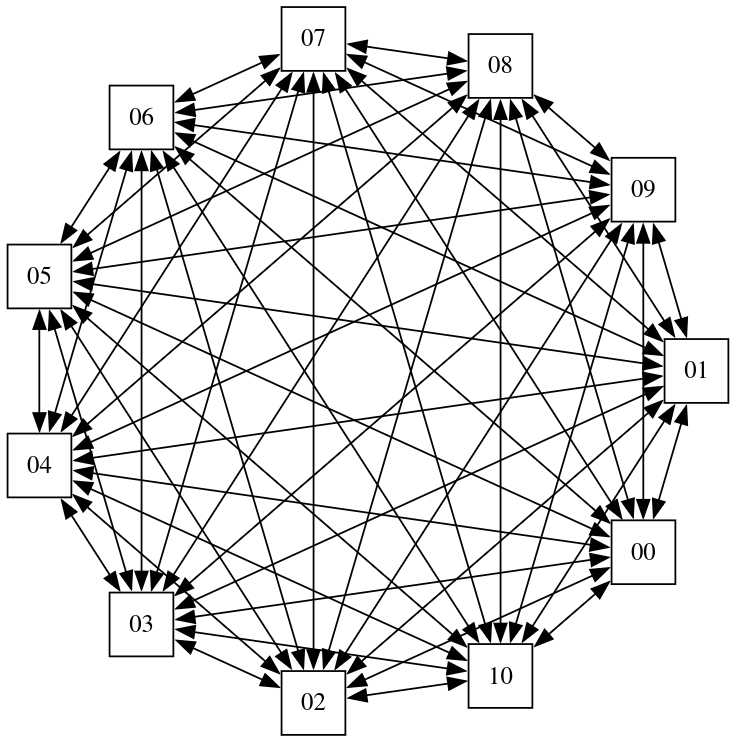
\includegraphics[width=0.8\linewidth]{figures/topologies/original.png}
\caption{Original Kubo -- topology}
\label{fig:original-topology}
\end{wrapfigure}

Since nodes decide on their own how to connect to each other, the
information about the topology was gathered after the benchmark. The nodes
formed a complete graph.

In case of the original Kubo implementation we notice a very smooth network
usage and disk usage. There are no nodes that have little to no activity. CPU
usage is consistent across nodes and is kept at around 50\% start to finish.

Figure \ref{fig:original-topology} displays how nodes are connected to each
other. Exact numbers for every metric are displayed in tables
\ref{tab:original-avg} and \ref{tab:original-total}. Table
\ref{tab:original-avg} contains metrics averages for every node. Similarly,
table \ref{tab:original-total} contains metrics totals for every node.

\textcolor{white}{.}\\\\\\\\\\\\

\begin{minipage}{0.5\linewidth}
\begin{figure}[H]
\captionsetup{justification=centering,width=0.8\linewidth}
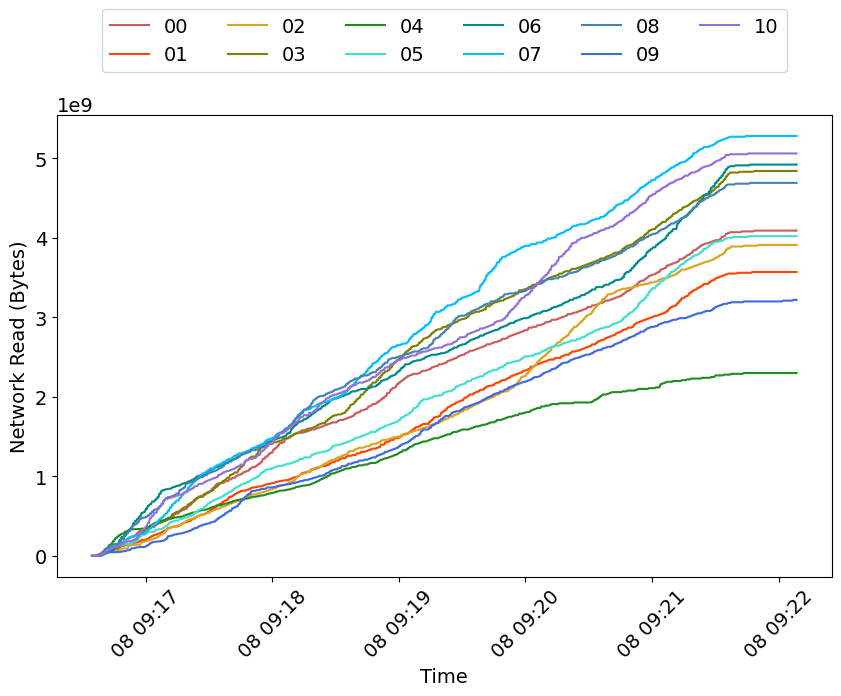
\includegraphics[width=\linewidth]{figures/original/net_read.png}
\caption{Original Kubo -- amount of bytes received over network}
\label{fig:original-net_read}
\end{figure}
\end{minipage}
\begin{minipage}{0.5\linewidth}
\begin{figure}[H]
\captionsetup{justification=centering,width=0.8\linewidth}
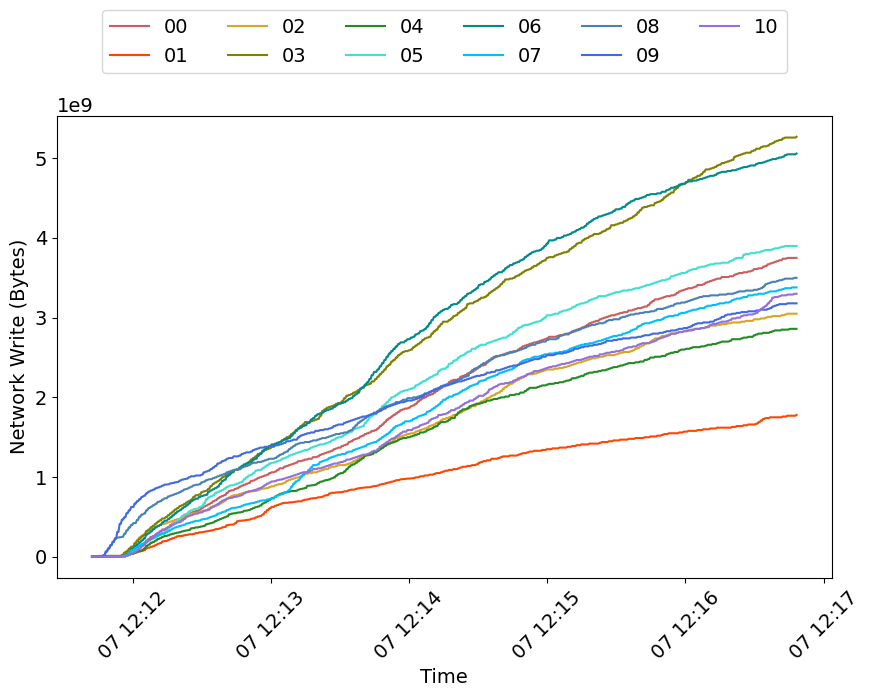
\includegraphics[width=\linewidth]{figures/original/net_write.png}
\caption{Original Kubo -- amount of bytes sent over network}
\label{fig:original-net_write}
\end{figure}
\end{minipage}

\begin{minipage}{0.5\linewidth}
\begin{figure}[H]
\captionsetup{justification=centering,width=0.8\linewidth}
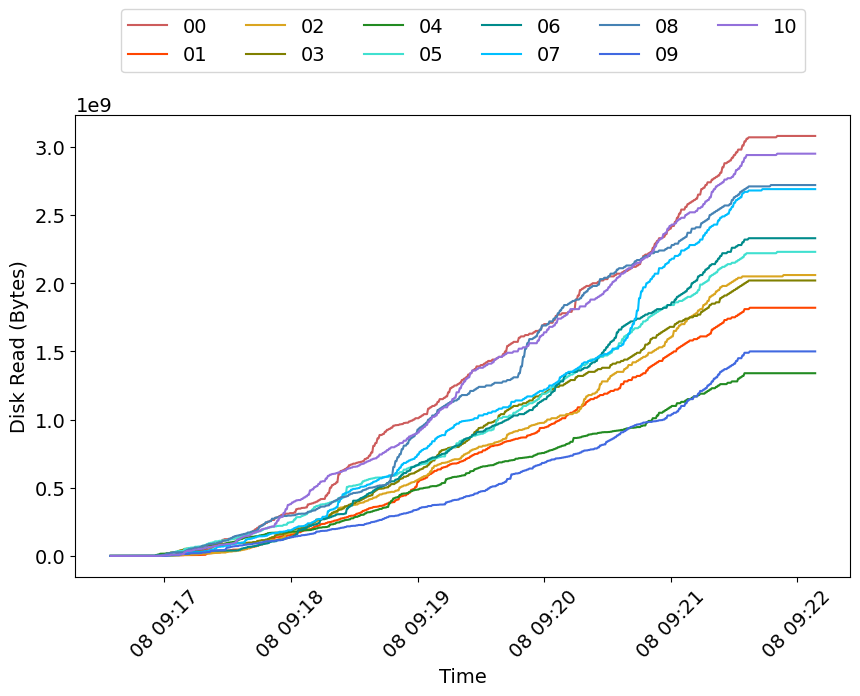
\includegraphics[width=\linewidth]{figures/original/blk_read.png}
\caption{Original Kubo -- amount of bytes read from disk}
\label{fig:original-blk_read}
\end{figure}
\end{minipage}
\begin{minipage}{0.5\linewidth}
\begin{figure}[H]
\captionsetup{justification=centering,width=0.8\linewidth}
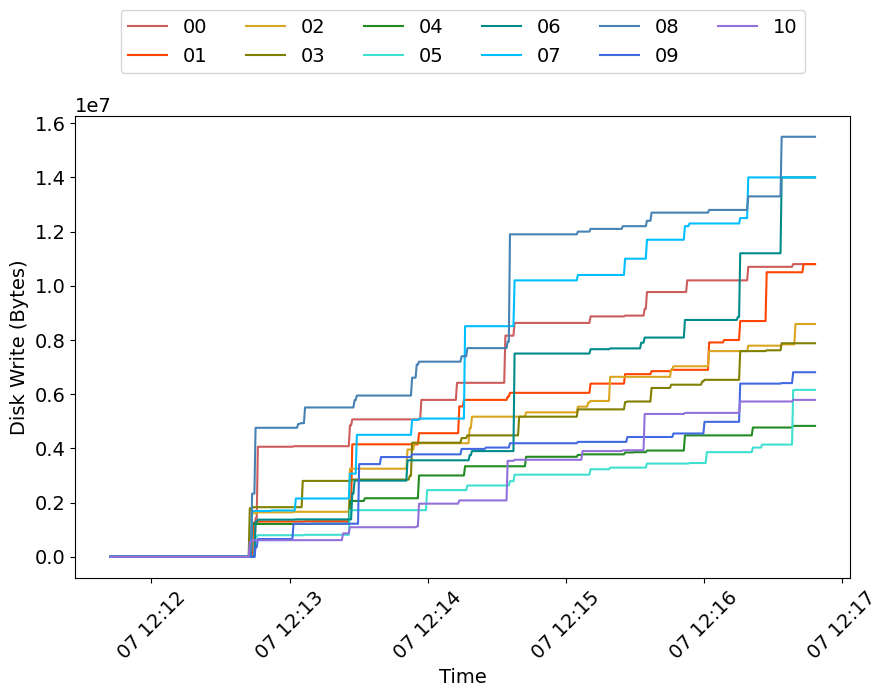
\includegraphics[width=\linewidth]{figures/original/blk_write.png}
\caption{Original Kubo -- amount of bytes written to disk}
\label{fig:original-blk_write}
\end{figure}
\end{minipage}

\begin{minipage}{0.5\linewidth}
\begin{figure}[H]
\captionsetup{justification=centering,width=0.8\linewidth}
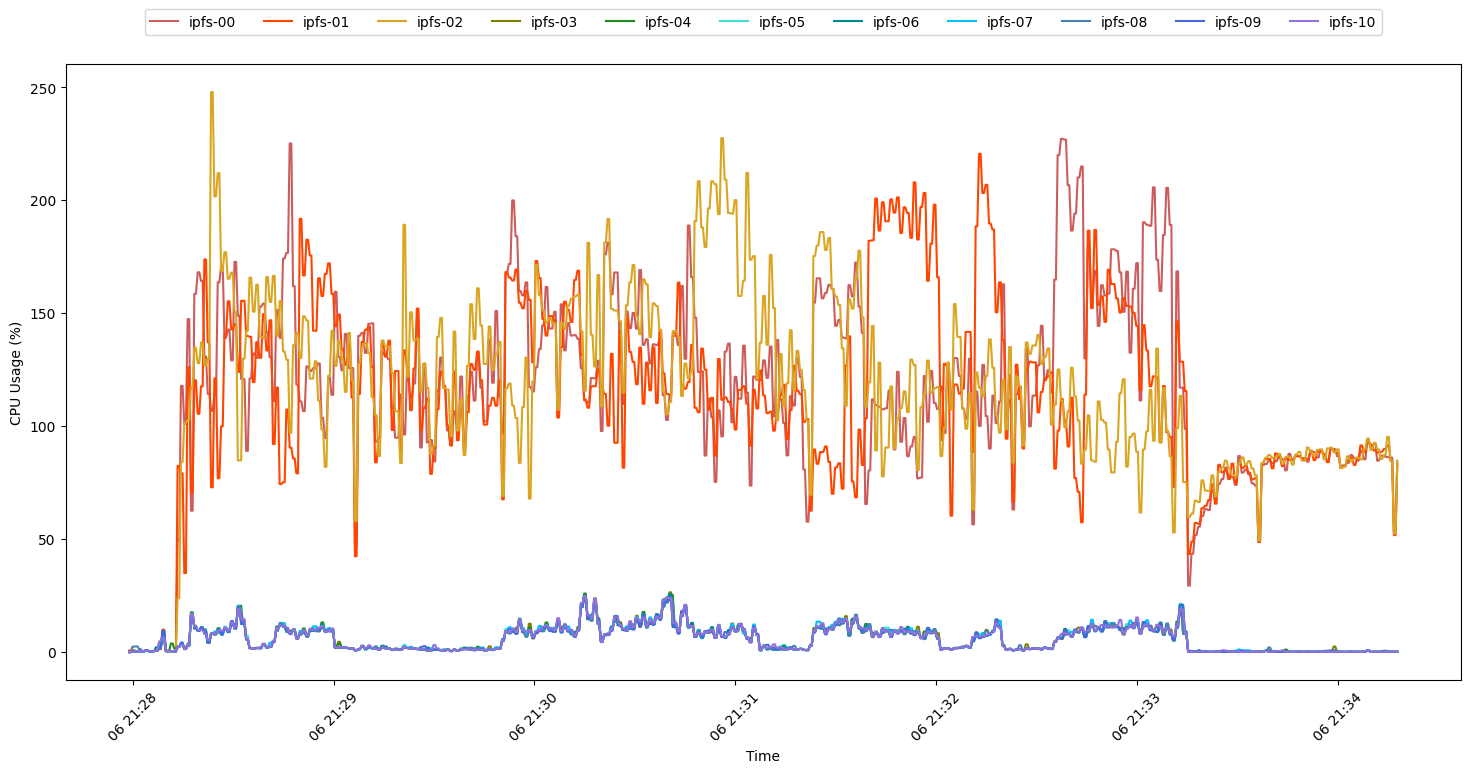
\includegraphics[width=\linewidth]{figures/original/cpu_usage.png}
\caption{Original Kubo -- CPU usage}
\label{fig:original-cpu_usage}
\end{figure}
\end{minipage}
\begin{minipage}{0.5\linewidth}
\begin{figure}[H]
\captionsetup{justification=centering,width=0.8\linewidth}
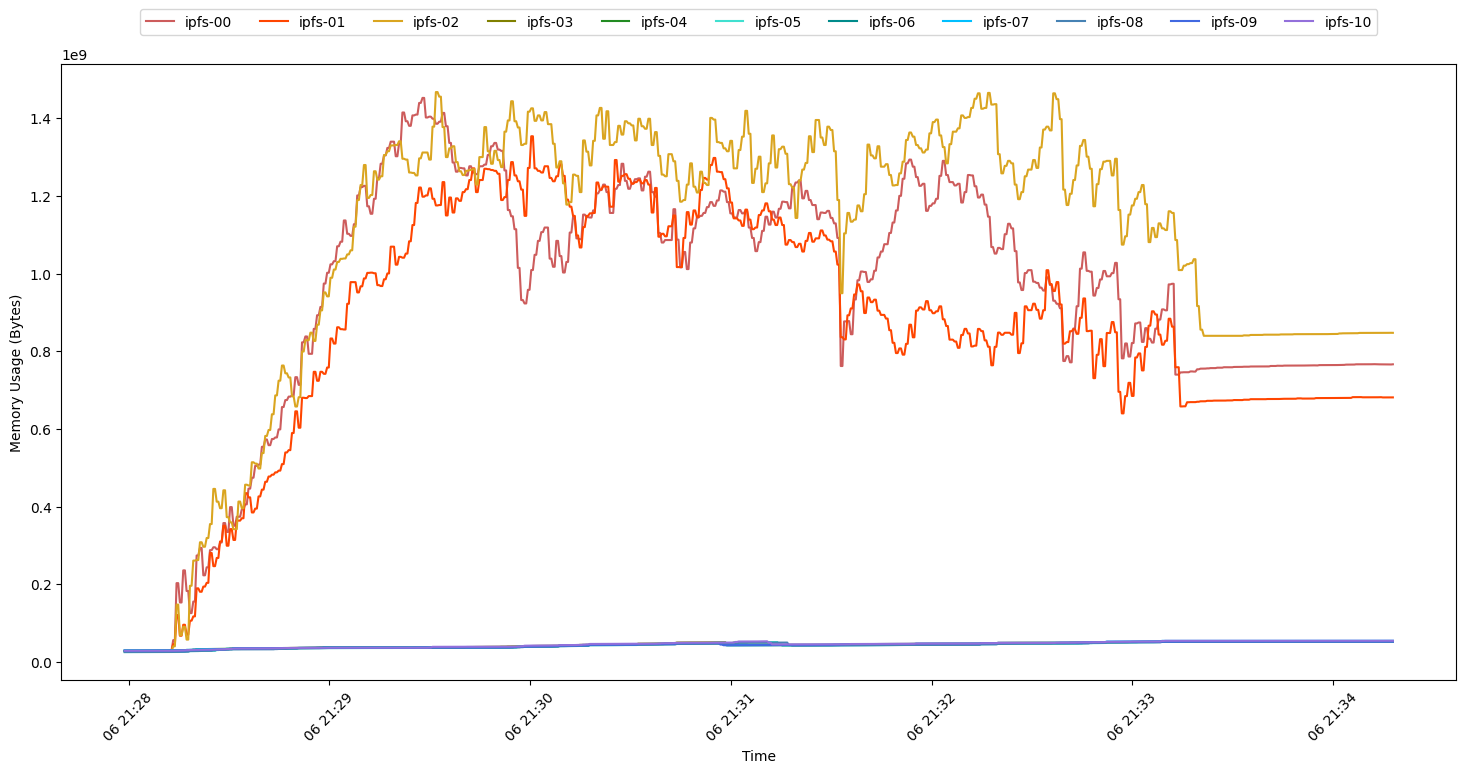
\includegraphics[width=\linewidth]{figures/original/mem_usage.png}
\caption{Original Kubo -- memory usage}
\label{fig:original-mem_usage}
\end{figure}
\end{minipage}

\begin{table}[H]
\begin{center}
\caption{Original Kubo -- metrics averages}
\label{tab:original-avg}
\begin{tabular}{|c|c|c|c|c|c|c|}
\hline
   & CPU usage & Memory usage & Disk read & Disk write & Network read & Network write\\
\hline
00 & 52.65\% & 341.87 MiB & 10.45 MiB/s & 12.31 MiB/s & 13.86 MiB/s & 25.96 MiB/s\\
01 & 48.03\% & 231.80 MiB & 6.13 MiB/s & 10.48 MiB/s & 12.03 MiB/s & 19.54 MiB/s\\
02 & 51.04\% & 244.21 MiB & 7.07 MiB/s & 11.66 MiB/s & 13.41 MiB/s & 22.57 MiB/s\\
03 & 50.74\% & 281.53 MiB & 6.90 MiB/s & 14.49 MiB/s & 16.54 MiB/s & 19.38 MiB/s\\
04 & 39.09\% & 178.95 MiB & 4.58 MiB/s & 7.45 MiB/s & 7.86 MiB/s & 14.63 MiB/s\\
05 & 50.60\% & 276.03 MiB & 7.51 MiB/s & 11.93 MiB/s & 13.54 MiB/s & 21.63 MiB/s\\
06 & 52.70\% & 279.56 MiB & 7.85 MiB/s & 14.69 MiB/s & 16.58 MiB/s & 20.69 MiB/s\\
07 & 55.05\% & 318.10 MiB & 9.13 MiB/s & 16.09 MiB/s & 17.92 MiB/s & 23.42 MiB/s\\
08 & 53.53\% & 294.36 MiB & 9.17 MiB/s & 13.48 MiB/s & 15.80 MiB/s & 23.01 MiB/s\\
09 & 45.17\% & 197.42 MiB & 5.09 MiB/s & 9.60 MiB/s & 10.93 MiB/s & 15.98 MiB/s\\
10 & 56.59\% & 341.36 MiB & 9.94 MiB/s & 14.93 MiB/s & 17.05 MiB/s & 27.06 MiB/s\\
\hline
\end{tabular}
\end{center}
\end{table}

\begin{table}[H]
\begin{center}
\caption{Original Kubo -- metrics totals}
\label{tab:original-total}
\begin{tabular}{|c|c|c|c|c|c|c|}
\hline
   & Disk read & Disk write & Network read & Network write\\
\hline
00 & 2.87 GiB & 3.38 GiB & 3.81 GiB & 7.12 GiB\\
01 & 1.70 GiB & 2.90 GiB & 3.32 GiB & 5.40 GiB\\
02 & 1.92 GiB & 3.17 GiB & 3.64 GiB & 6.13 GiB\\
03 & 1.88 GiB & 3.95 GiB & 4.51 GiB & 5.28 GiB\\
04 & 1.25 GiB & 2.03 GiB & 2.14 GiB & 3.99 GiB\\
05 & 2.08 GiB & 3.30 GiB & 3.74 GiB & 5.98 GiB\\
06 & 2.17 GiB & 4.06 GiB & 4.58 GiB & 5.72 GiB\\
07 & 2.51 GiB & 4.41 GiB & 4.92 GiB & 6.43 GiB\\
08 & 2.53 GiB & 3.73 GiB & 4.37 GiB & 6.36 GiB\\
09 & 1.40 GiB & 2.64 GiB & 3.00 GiB & 4.39 GiB\\
10 & 2.75 GiB & 4.13 GiB & 4.71 GiB & 7.48 GiB\\
\hline
\end{tabular}
\end{center}
\end{table}



\newpage
\subsection{Case 2: Ring Topology}

\begin{wrapfigure}{r}{0.5\textwidth}
\centering
\captionsetup{justification=centering,width=0.6\linewidth}
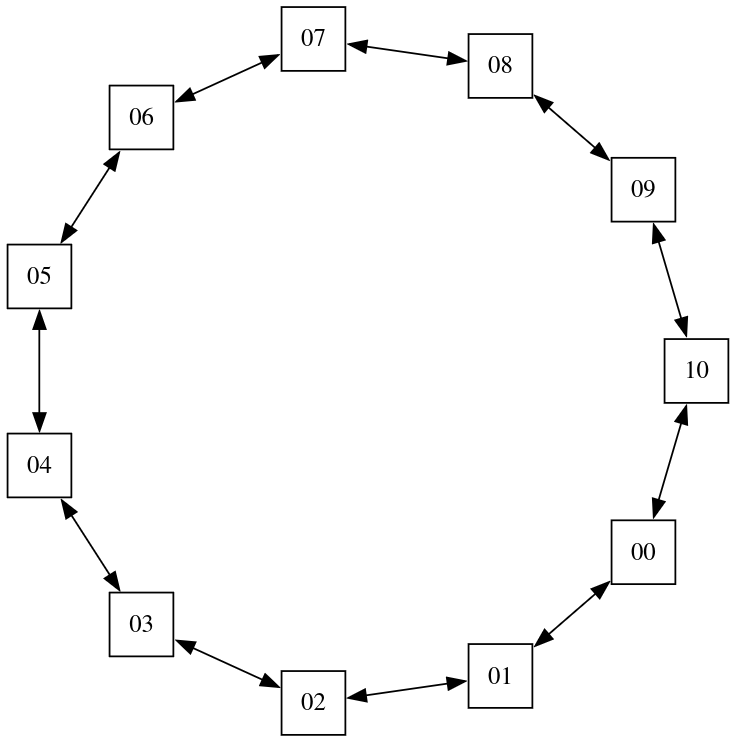
\includegraphics[width=0.8\linewidth]{figures/topologies/ring.png}
\caption{Ring -- topology}
\label{fig:ring-topology}

\end{wrapfigure}
It can be observed in figure \ref{fig:ring-blk_read} that disk reads don't
happen until much later in the benchmarking process. We think that is because
of the way files propagate through the network. Since a node is unlikely to be
able to talk directly to the one that has the file, it has to wait until
eventually one of its neighbours has it. This way, many initial requests for
the file just time out and we see a big interval of disk read inactivity in the
beginning.

On top of that, all metrics exhibit very uneven behaviour between nodes. There
are some nodes that eventually serve a lot of files and others that have very
little activity. The ones that are the most active are in a continuous range in
the ring, namely the nodes \verb|07| through \verb|00|. It might just happen
that by chance more files were uploaded and downloaded in the beginning
specifically in that part of the ring, which would make the file spread sooner
there.

Finally, the CPU usage is very spiky and also comes in bursts as can be seen in
figure \ref{fig:ring-cpu_usage}. We think that the silent periods are caused by
the fact that any given node has only two neighbours and it cannot directly
reach the node that has the file, so it has to wait for one of the neighbours
to get the file. The spikes are probably happening when the node finally gets
the file. Since there might be many clients waiting for the same file from the
same node, Kubo has to process and send it to all of them at the same time once
the file becomes available, hence the sudden increase in CPU usage, after which
it also quickly decreases.

Figure \ref{fig:ring-topology} displays how nodes are connected to each other.
Exact numbers for every metric are displayed in tables \ref{tab:ring-avg} and
\ref{tab:ring-total}. Table \ref{tab:ring-avg} contains metrics averages for
every node. Similarly, table \ref{tab:ring-total} contains metrics totals for
every node.

\begin{minipage}{0.5\linewidth}
\begin{figure}[H]
\captionsetup{justification=centering,width=0.8\linewidth}
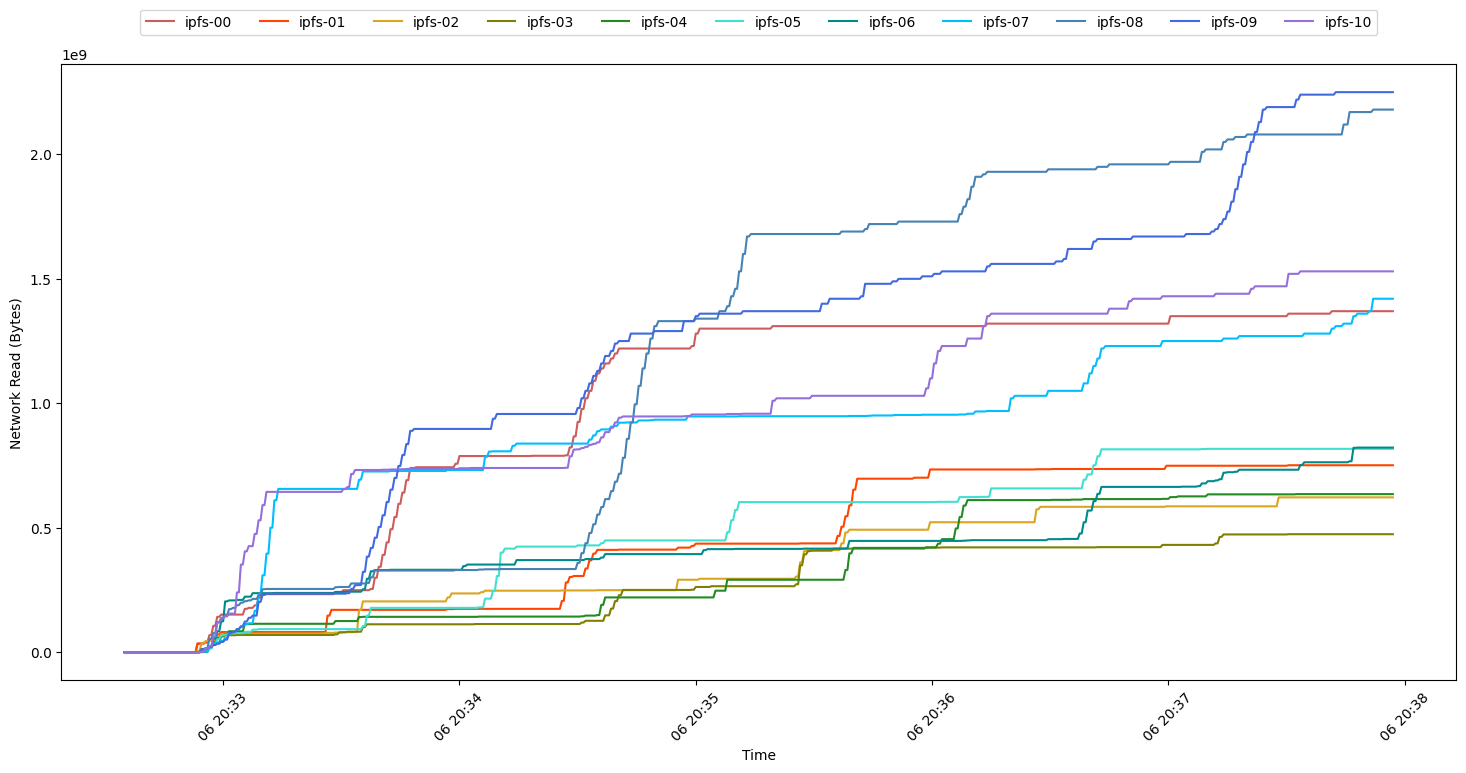
\includegraphics[width=\linewidth]{figures/ring/net_read.png}
\caption{Ring topology -- amount of bytes received over network}
\label{fig:ring-net_read}
\end{figure}
\end{minipage}
\begin{minipage}{0.5\linewidth}
\begin{figure}[H]
\captionsetup{justification=centering,width=0.8\linewidth}
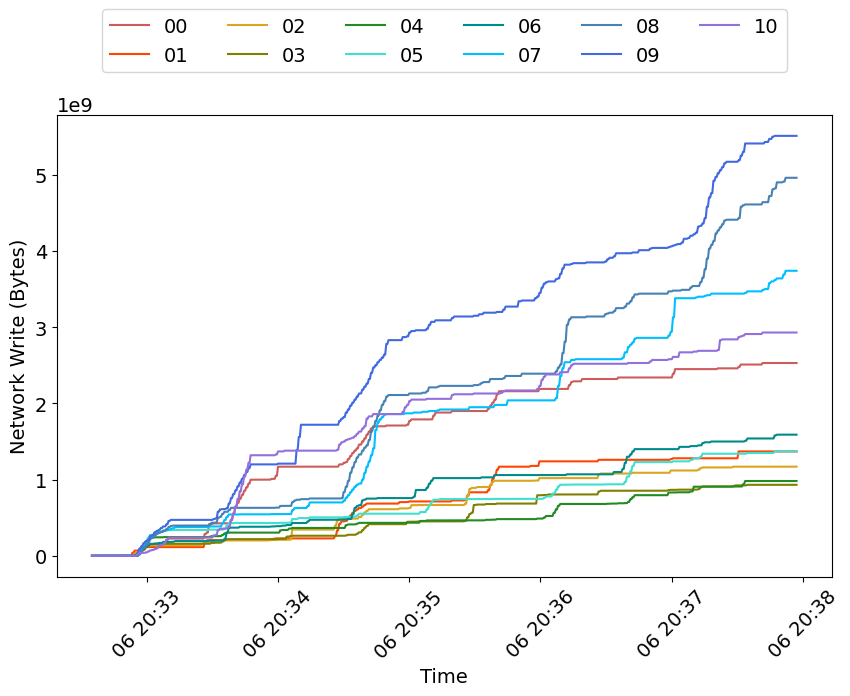
\includegraphics[width=\linewidth]{figures/ring/net_write.png}
\caption{Ring topology -- amount of bytes sent over network}
\label{fig:ring-net_write}
\end{figure}
\end{minipage}

\begin{minipage}{0.5\linewidth}
\begin{figure}[H]
\captionsetup{justification=centering,width=0.8\linewidth}
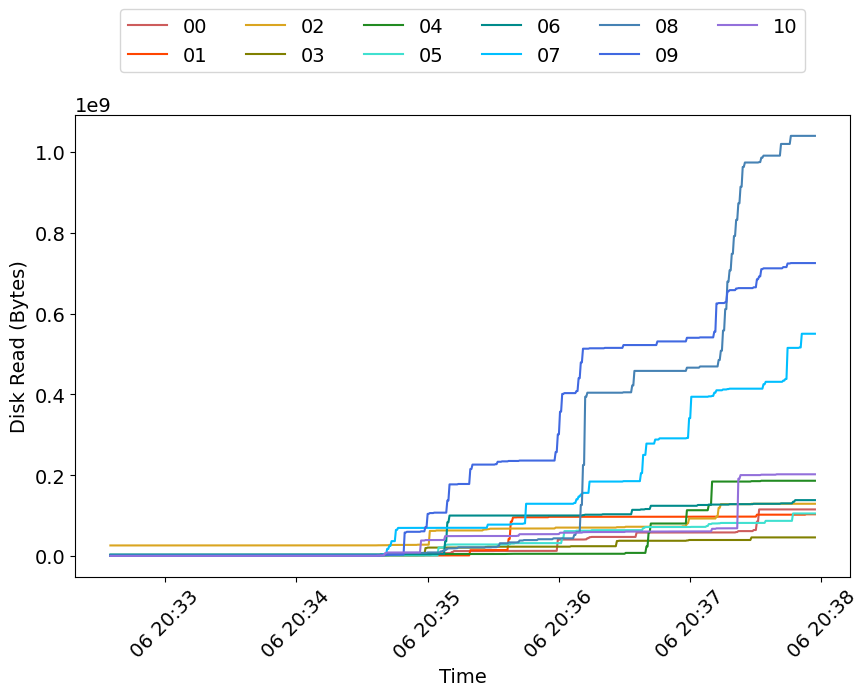
\includegraphics[width=\linewidth]{figures/ring/blk_read.png}
\caption{Ring topology -- amount of bytes read from disk}
\label{fig:ring-blk_read}
\end{figure}
\end{minipage}
\begin{minipage}{0.5\linewidth}
\begin{figure}[H]
\captionsetup{justification=centering,width=0.8\linewidth}
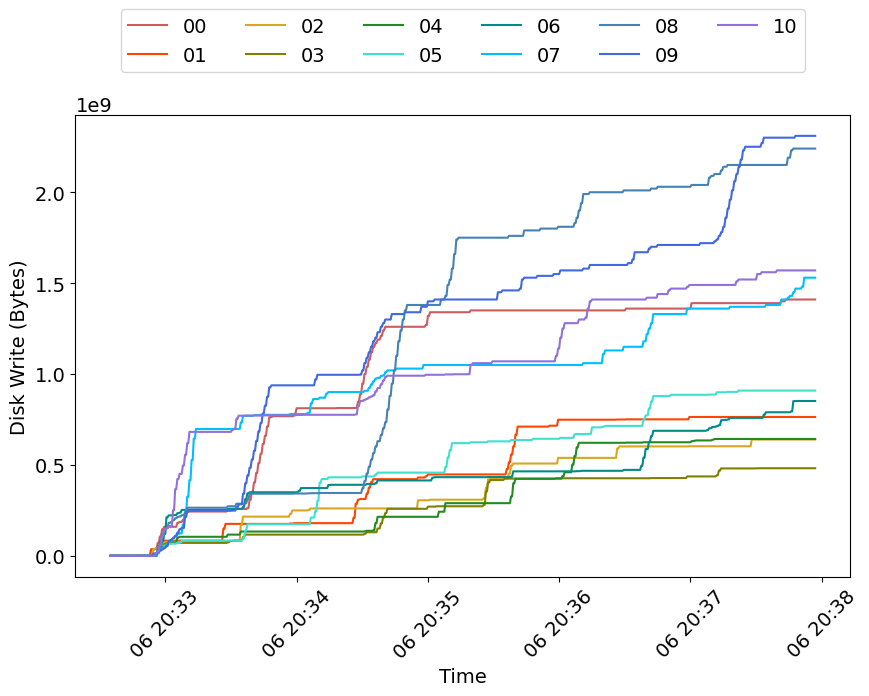
\includegraphics[width=\linewidth]{figures/ring/blk_write.png}
\caption{Ring topology -- amount of bytes written to disk}
\label{fig:ring-blk_write}
\end{figure}
\end{minipage}

\begin{minipage}{0.5\linewidth}
\begin{figure}[H]
\captionsetup{justification=centering,width=0.8\linewidth}
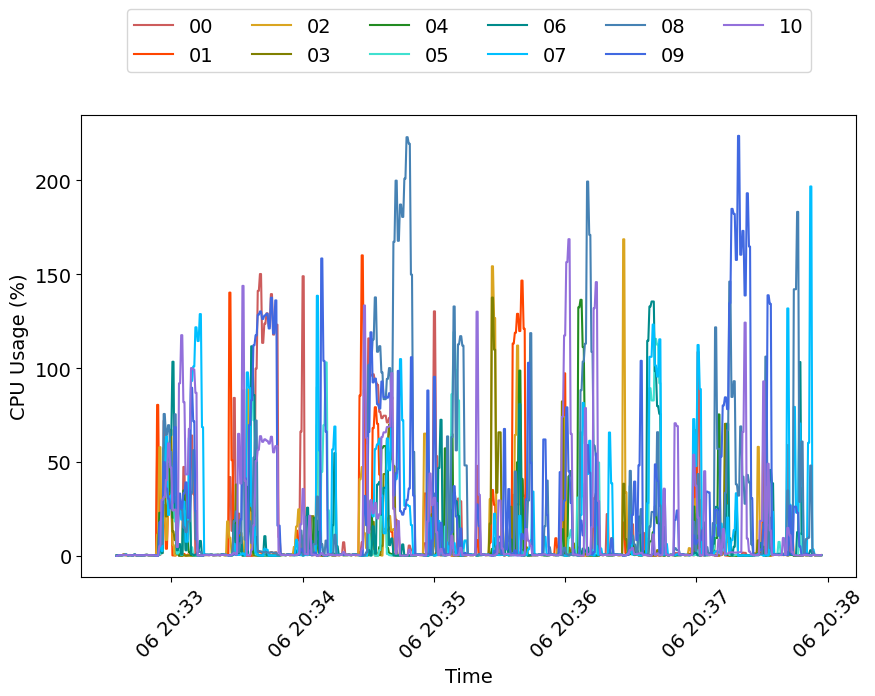
\includegraphics[width=\linewidth]{figures/ring/cpu_usage.png}
\caption{Ring topology -- CPU usage}
\label{fig:ring-cpu_usage}
\end{figure}
\end{minipage}
\begin{minipage}{0.5\linewidth}
\begin{figure}[H]
\captionsetup{justification=centering,width=0.8\linewidth}
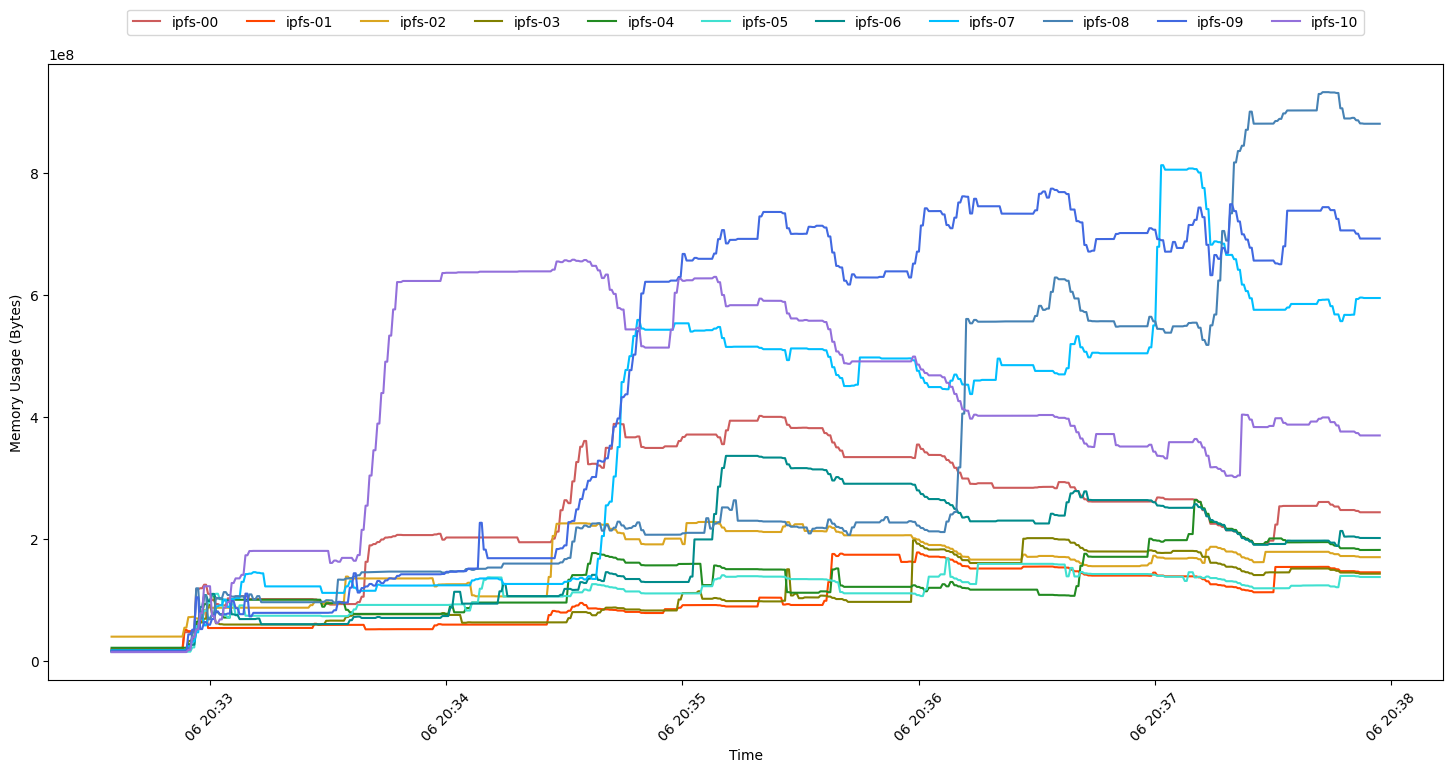
\includegraphics[width=\linewidth]{figures/ring/mem_usage.png}
\caption{Ring topology -- memory usage}
\label{fig:ring-mem_usage}
\end{figure}
\end{minipage}

\begin{table}[H]
\begin{center}
\caption{Ring -- metrics averages}
\label{tab:ring-avg}
\begin{tabular}{|c|c|c|c|c|c|c|}
\hline
   & CPU usage & Memory usage & Disk read & Disk write & Network read & Network write\\
\hline
00 & 13.85\% & 232.01 MiB & 407.22 KiB/s & 4.92 MiB/s & 4.79 MiB/s & 8.84 MiB/s\\
01 & 7.59\% & 97.67 MiB & 369.74 KiB/s & 2.69 MiB/s & 2.64 MiB/s & 4.82 MiB/s\\
02 & 6.16\% & 149.98 MiB & 371.89 KiB/s & 2.25 MiB/s & 2.19 MiB/s & 4.12 MiB/s\\
03 & 5.13\% & 104.34 MiB & 164.39 KiB/s & 1.70 MiB/s & 1.67 MiB/s & 3.28 MiB/s\\
04 & 6.15\% & 122.33 MiB & 664.46 KiB/s & 2.26 MiB/s & 2.23 MiB/s & 3.46 MiB/s\\
05 & 7.67\% & 107.04 MiB & 372.38 KiB/s & 3.15 MiB/s & 2.83 MiB/s & 4.75 MiB/s\\
06 & 8.60\% & 167.83 MiB & 482.97 KiB/s & 2.99 MiB/s & 2.88 MiB/s & 5.57 MiB/s\\
07 & 15.55\% & 351.82 MiB & 1.92 MiB/s & 5.34 MiB/s & 4.96 MiB/s & 13.06 MiB/s\\
08 & 25.18\% & 317.90 MiB & 3.63 MiB/s & 7.82 MiB/s & 7.62 MiB/s & 17.33 MiB/s\\
09 & 26.76\% & 441.80 MiB & 2.53 MiB/s & 8.07 MiB/s & 7.86 MiB/s & 19.25 MiB/s\\
10 & 15.63\% & 393.72 MiB & 727.78 KiB/s & 5.52 MiB/s & 5.38 MiB/s & 10.31 MiB/s\\
\hline
\end{tabular}
\end{center}
\end{table}

\begin{table}[H]
\begin{center}
\caption{Ring -- metrics totals}
\label{tab:ring-total}
\begin{tabular}{|c|c|c|c|c|c|c|}
\hline
   & Disk read & Disk write & Network read & Network write\\
\hline
00 & 109.67 MiB & 1.31 GiB & 1.28 GiB & 2.36 GiB\\
01 & 98.23 MiB & 728.61 MiB & 716.21 MiB & 1.28 GiB\\
02 & 123.02 MiB & 610.35 MiB & 593.19 MiB & 1.09 GiB\\
03 & 43.58 MiB & 459.67 MiB & 452.04 MiB & 888.82 MiB\\
04 & 177.38 MiB & 613.21 MiB & 605.58 MiB & 936.51 MiB\\
05 & 100.14 MiB & 866.89 MiB & 779.15 MiB & 1.28 GiB\\
06 & 131.61 MiB & 812.53 MiB & 783.92 MiB & 1.48 GiB\\
07 & 524.52 MiB & 1.42 GiB & 1.32 GiB & 3.48 GiB\\
08 & 991.82 MiB & 2.09 GiB & 2.03 GiB & 4.62 GiB\\
09 & 691.41 MiB & 2.15 GiB & 2.10 GiB & 5.13 GiB\\
10 & 192.64 MiB & 1.46 GiB & 1.42 GiB & 2.73 GiB\\
\hline
\end{tabular}
\end{center}
\end{table}



\newpage
\subsection{Case 3: Grid Topology}

\begin{wrapfigure}{r}{0.5\textwidth}
\centering
\captionsetup{justification=centering,width=0.5\linewidth}
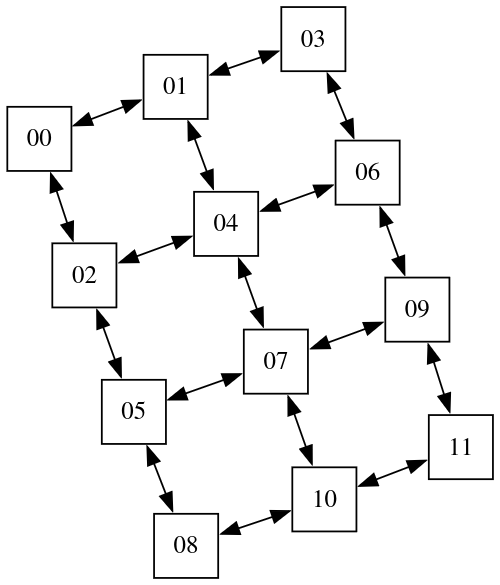
\includegraphics[width=0.7\linewidth]{figures/topologies/grid.png}
\caption{Grid -- topology}
\label{fig:grid-topology}
\end{wrapfigure}

Grid topology shows a similar overall behaviour to ring topology, except one
big difference in terms of disk usage. In case of ring topology there are
several very distinctive spikes in both reading and writing, whereas in grid
topology the spikes are much smaller and the usage is smoother generally. We
think that is thanks to the fact that nodes have more neighbours and so if a
file becomes available at one node, then more other nodes can get access to it.
We also observe that the nodes with the least amount of activity are usually
the ones with the least amount of neighbours, namely: the nodes located in the
corners of the grid.

Figure \ref{fig:grid-topology} displays how nodes are connected to each other.
Exact numbers for every metric are displayed in tables \ref{tab:grid-avg} and
\ref{tab:grid-total}. Table \ref{tab:grid-avg} contains metrics averages for
every node. Similarly, table \ref{tab:grid-total} contains metrics totals for
every node.

\textcolor{white}{.}\\\\

\begin{minipage}{0.5\linewidth}
\begin{figure}[H]
\captionsetup{justification=centering,width=0.8\linewidth}
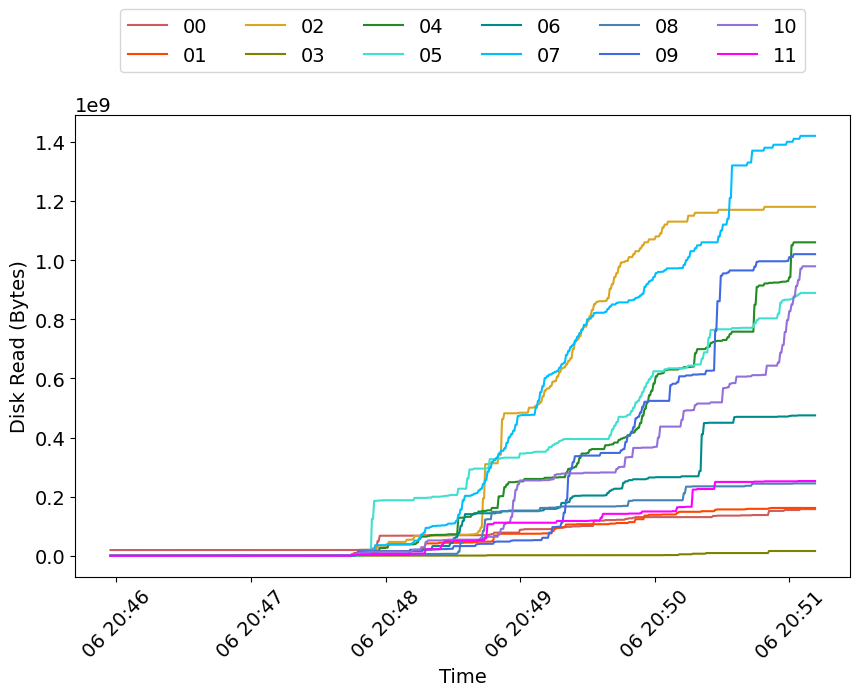
\includegraphics[width=\linewidth]{figures/grid/blk_read.png}
\caption{Grid topology -- amount of bytes read from disk}
\label{fig:grid-net_read}
\end{figure}
\end{minipage}
\begin{minipage}{0.5\linewidth}
\begin{figure}[H]
\captionsetup{justification=centering,width=0.8\linewidth}
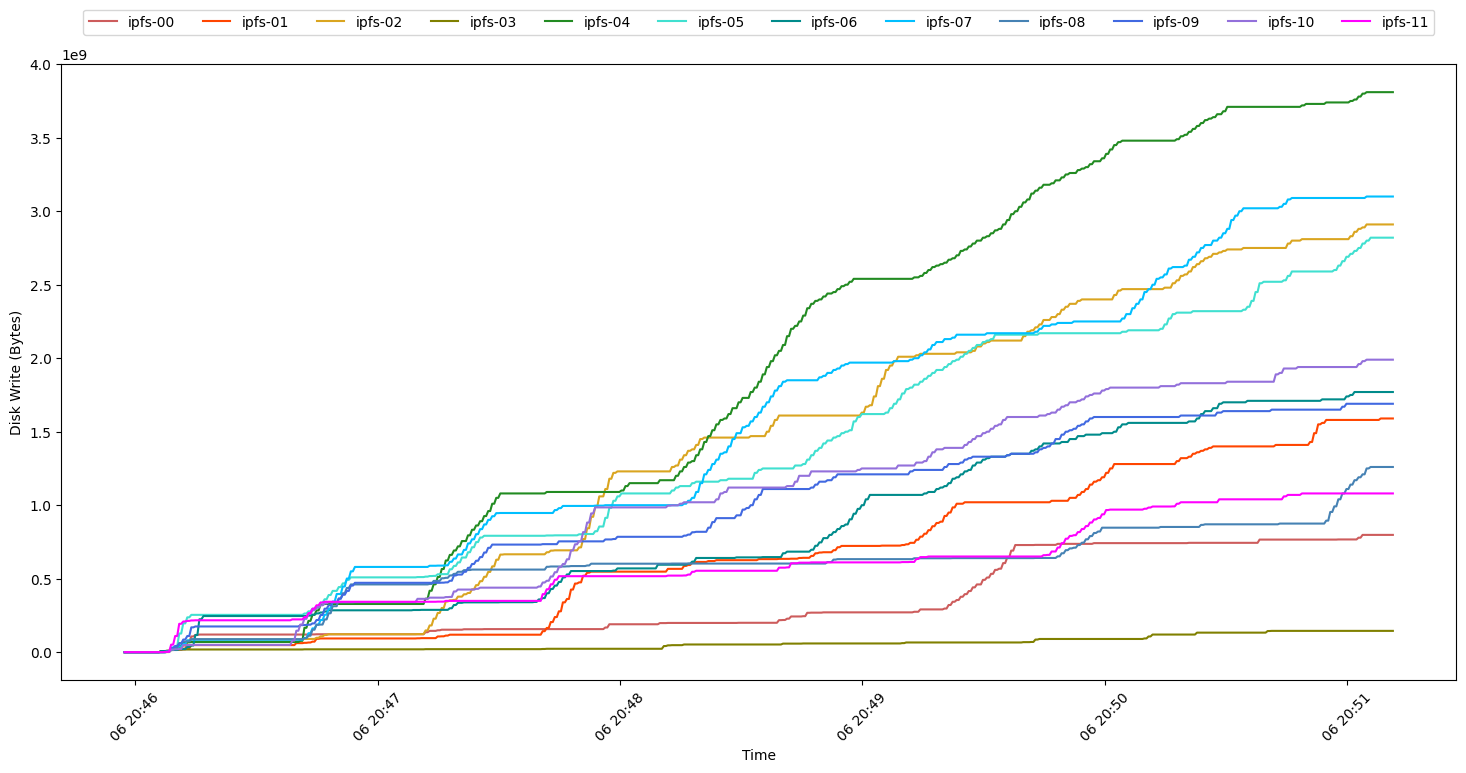
\includegraphics[width=\linewidth]{figures/grid/blk_write.png}
\caption{Grid topology -- amount of bytes written to disk}
\label{fig:grid-net_write}
\end{figure}
\end{minipage}

\begin{minipage}{0.5\linewidth}
\begin{figure}[H]
\captionsetup{justification=centering,width=0.8\linewidth}
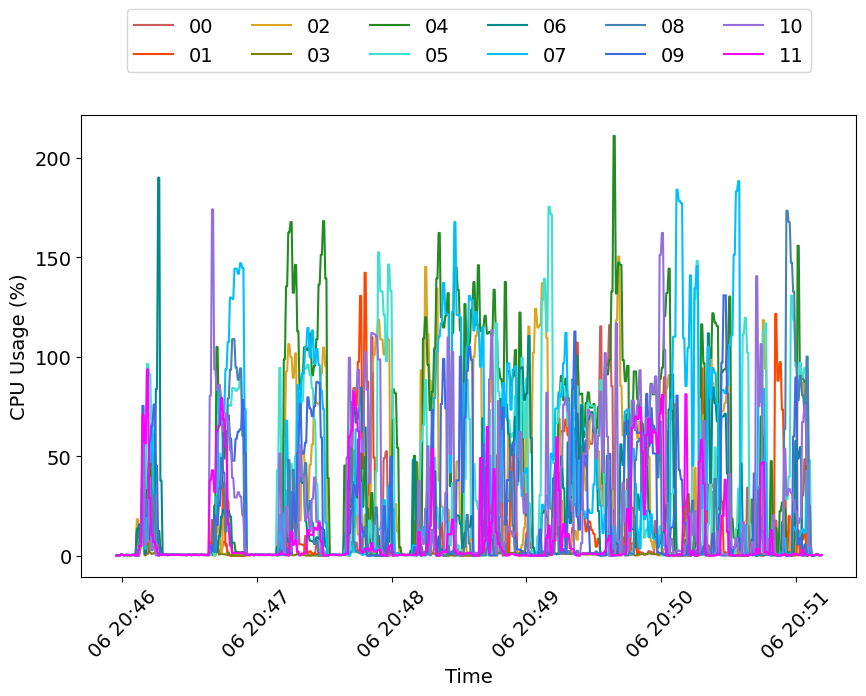
\includegraphics[width=\linewidth]{figures/grid/cpu_usage.png}
\caption{Grid topology -- CPU usage}
\label{fig:grid-blk_read}
\end{figure}
\end{minipage}
\begin{minipage}{0.5\linewidth}
\begin{figure}[H]
\captionsetup{justification=centering,width=0.8\linewidth}
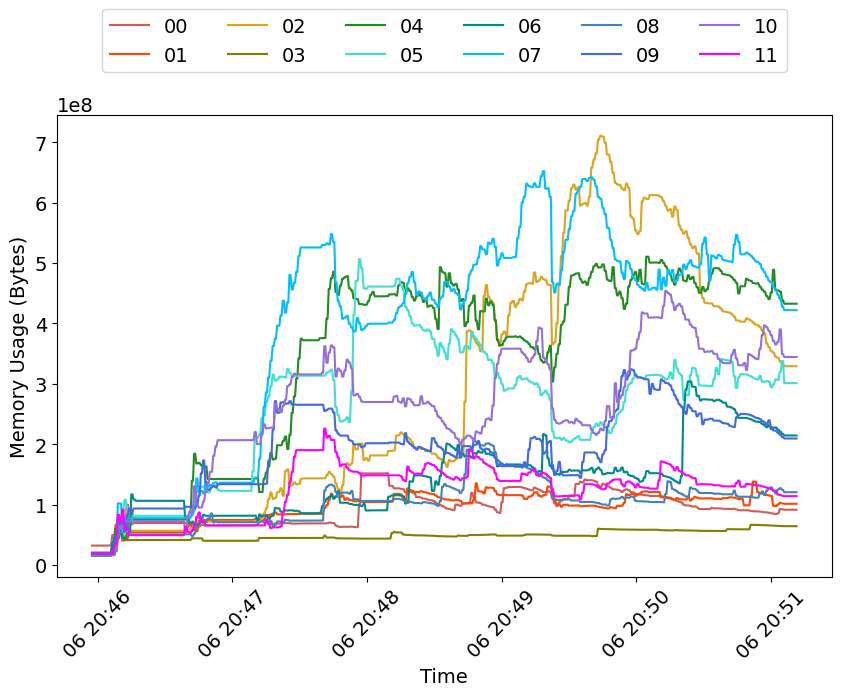
\includegraphics[width=\linewidth]{figures/grid/mem_usage.png}
\caption{Grid topology -- memory usage}
\label{fig:grid-blk_write}
\end{figure}
\end{minipage}

\begin{minipage}{0.5\linewidth}
\begin{figure}[H]
\captionsetup{justification=centering,width=0.8\linewidth}
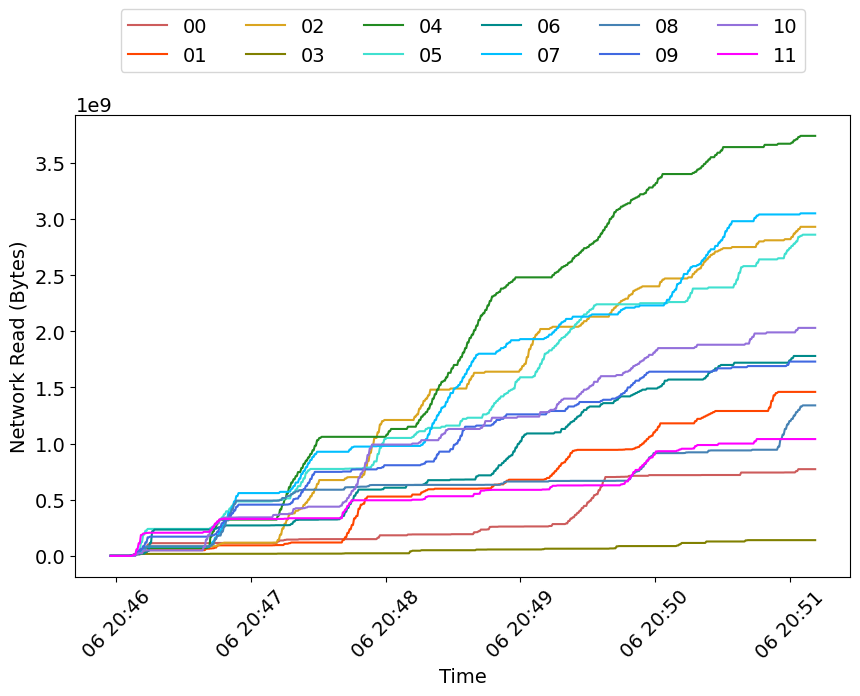
\includegraphics[width=\linewidth]{figures/grid/net_read.png}
\caption{Grid topology -- amount of bytes received over network}
\label{fig:grid-cpu_usage}
\end{figure}
\end{minipage}
\begin{minipage}{0.5\linewidth}
\begin{figure}[H]
\captionsetup{justification=centering,width=0.8\linewidth}
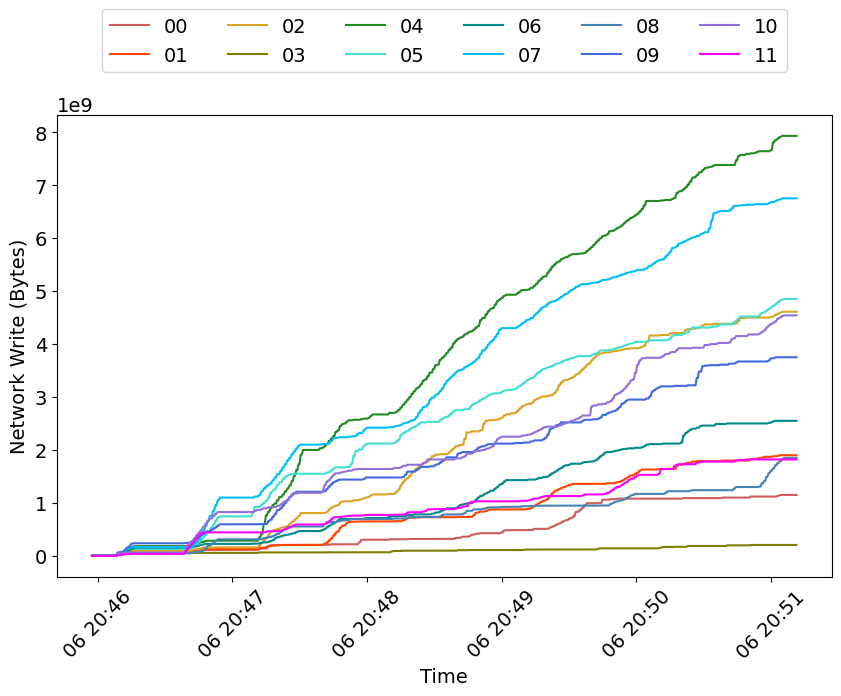
\includegraphics[width=\linewidth]{figures/grid/net_write.png}
\caption{Grid topology -- amount of bytes sent over network}
\label{fig:grid-mem_usage}
\end{figure}
\end{minipage}

\begin{table}[H]
\begin{center}
\caption{Grid -- metrics averages}
\label{tab:grid-avg}
\begin{tabular}{|c|c|c|c|c|c|c|}
\hline
   & CPU usage & Memory usage & Disk read & Disk write & Network read & Network write\\
\hline
00 & 7.50\% & 89.86 MiB & 519.83 KiB/s & 2.93 MiB/s & 2.83 MiB/s & 4.22 MiB/s\\
01 & 14.31\% & 90.63 MiB & 607.58 KiB/s & 5.83 MiB/s & 5.36 MiB/s & 6.97 MiB/s\\
02 & 32.36\% & 278.24 MiB & 4.33 MiB/s & 10.67 MiB/s & 10.75 MiB/s & 16.91 MiB/s\\
03 & 1.92\% & 46.29 MiB & 61.50 KiB/s & 545.95 KiB/s & 527.74 KiB/s & 776.68 KiB/s\\
04 & 49.78\% & 329.60 MiB & 3.87 MiB/s & 13.92 MiB/s & 13.67 MiB/s & 28.98 MiB/s\\
05 & 33.43\% & 252.92 MiB & 3.25 MiB/s & 10.30 MiB/s & 10.45 MiB/s & 17.72 MiB/s\\
06 & 18.93\% & 135.11 MiB & 1.72 MiB/s & 6.42 MiB/s & 6.45 MiB/s & 9.25 MiB/s\\
07 & 40.22\% & 374.35 MiB & 5.21 MiB/s & 11.37 MiB/s & 11.19 MiB/s & 24.76 MiB/s\\
08 & 12.61\% & 97.96 MiB & 920.08 KiB/s & 4.62 MiB/s & 4.91 MiB/s & 6.79 MiB/s\\
09 & 20.19\% & 182.12 MiB & 3.73 MiB/s & 6.17 MiB/s & 6.32 MiB/s & 13.70 MiB/s\\
10 & 25.13\% & 248.15 MiB & 3.59 MiB/s & 7.30 MiB/s & 7.45 MiB/s & 16.65 MiB/s\\
11 & 10.53\% & 115.71 MiB & 952.72 KiB/s & 3.98 MiB/s & 3.83 MiB/s & 6.70 MiB/s\\
\hline
\end{tabular}
\end{center}
\end{table}

\begin{table}[H]
\begin{center}
\caption{Grid -- metrics totals}
\label{tab:grid-total}
\begin{tabular}{|c|c|c|c|c|c|c|}
\hline
   & Disk read & Disk write & Network read & Network write\\
\hline
00 & 150.68 MiB & 761.03 MiB & 736.24 MiB & 1.07 GiB\\
01 & 154.50 MiB & 1.48 GiB & 1.36 GiB & 1.77 GiB\\
02 & 1.10 GiB & 2.71 GiB & 2.73 GiB & 4.29 GiB\\
03 & 15.64 MiB & 138.28 MiB & 133.51 MiB & 196.46 MiB\\
04 & 1010.89 MiB & 3.55 GiB & 3.48 GiB & 7.39 GiB\\
05 & 847.82 MiB & 2.63 GiB & 2.66 GiB & 4.52 GiB\\
06 & 453.00 MiB & 1.65 GiB & 1.66 GiB & 2.37 GiB\\
07 & 1.32 GiB & 2.89 GiB & 2.84 GiB & 6.29 GiB\\
08 & 233.65 MiB & 1.17 GiB & 1.25 GiB & 1.72 GiB\\
09 & 972.75 MiB & 1.57 GiB & 1.61 GiB & 3.49 GiB\\
10 & 933.65 MiB & 1.85 GiB & 1.89 GiB & 4.23 GiB\\
11 & 241.28 MiB & 1.01 GiB & 991.82 MiB & 1.70 GiB\\
\hline
\end{tabular}
\end{center}
\end{table}



\newpage
\subsection{Case 4: Random Graph Topology}

\begin{wrapfigure}{r}{0.5\textwidth}
\centering
\captionsetup{justification=centering,width=0.8\linewidth}
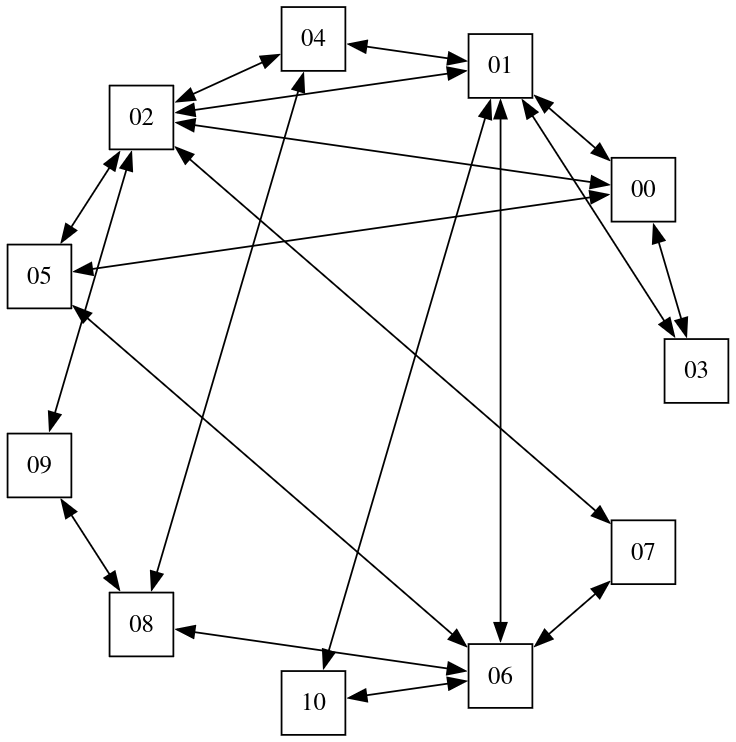
\includegraphics[width=0.7\linewidth]{figures/topologies/graph-random.png}
\caption{Random graph -- topology}
\label{fig:graph-random-topology}
\end{wrapfigure}

Results for random graph topology are similar in a way to the ones for grid
topology. The same uneven load is observed in case of disk I/O as well as
network I/O, but in contrast to a grid, in a random graph there are little to
no spikes being observed. The big difference is CPU usage, which is not bursty
and more or less consistent across nodes, but it's spiky. Also, we observe that
the nodes that get the most network traffic are usually the ones that have many
neighbours, for example: nodes \verb|06|, \verb|01|, \verb|02|.

Figure \ref{fig:graph-random-topology} displays how nodes are connected to each
other. Exact numbers for every metric are displayed in tables
\ref{tab:graph-random-avg} and \ref{tab:graph-random-total}. Table
\ref{tab:graph-random-avg} contains metrics averages for every node. Similarly,
table \ref{tab:graph-random-total} contains metrics totals for every node.

\textcolor{white}{.}\\

\begin{minipage}{0.5\linewidth}
\begin{figure}[H]
\captionsetup{justification=centering,width=0.8\linewidth}
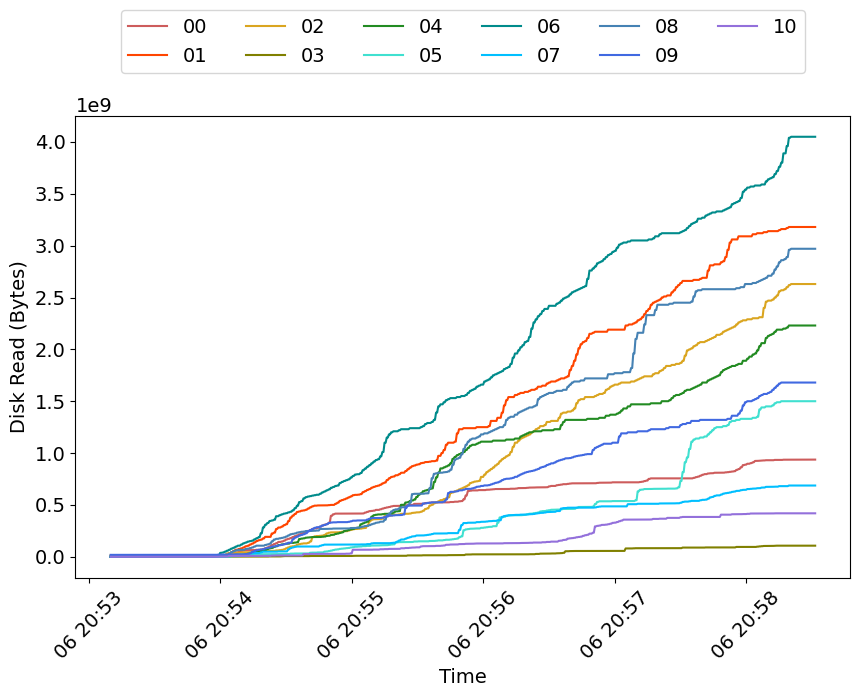
\includegraphics[width=\linewidth]{figures/graph-random/blk_read.png}
\caption{Random graph topology -- amount of bytes read from disk}
\label{fig:graph-random-net_read}
\end{figure}
\end{minipage}
\begin{minipage}{0.5\linewidth}
\begin{figure}[H]
\captionsetup{justification=centering,width=0.8\linewidth}
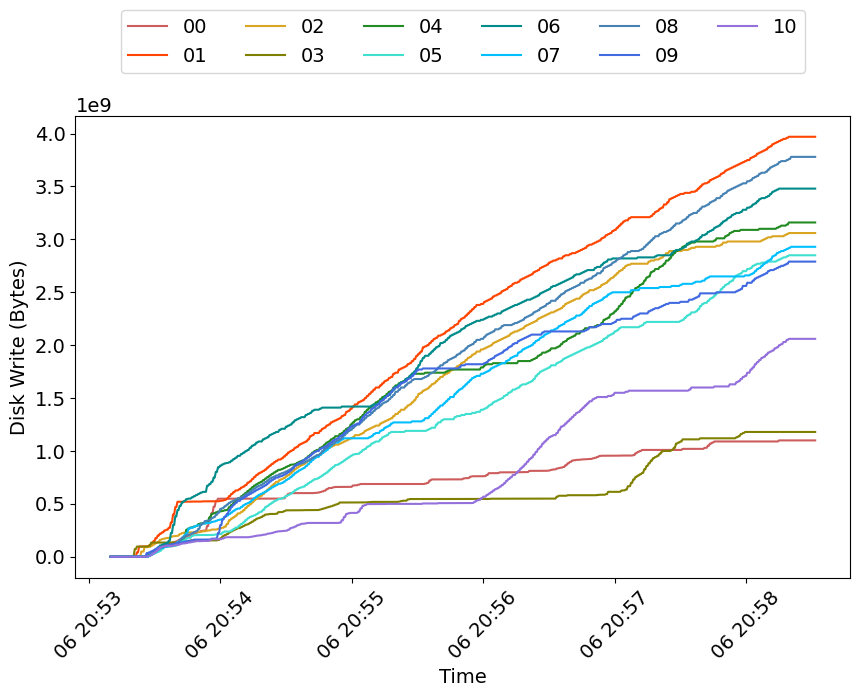
\includegraphics[width=\linewidth]{figures/graph-random/blk_write.png}
\caption{Random graph topology -- amount of bytes written to disk}
\label{fig:graph-random-net_write}
\end{figure}
\end{minipage}

\begin{minipage}{0.5\linewidth}
\begin{figure}[H]
\captionsetup{justification=centering,width=0.8\linewidth}
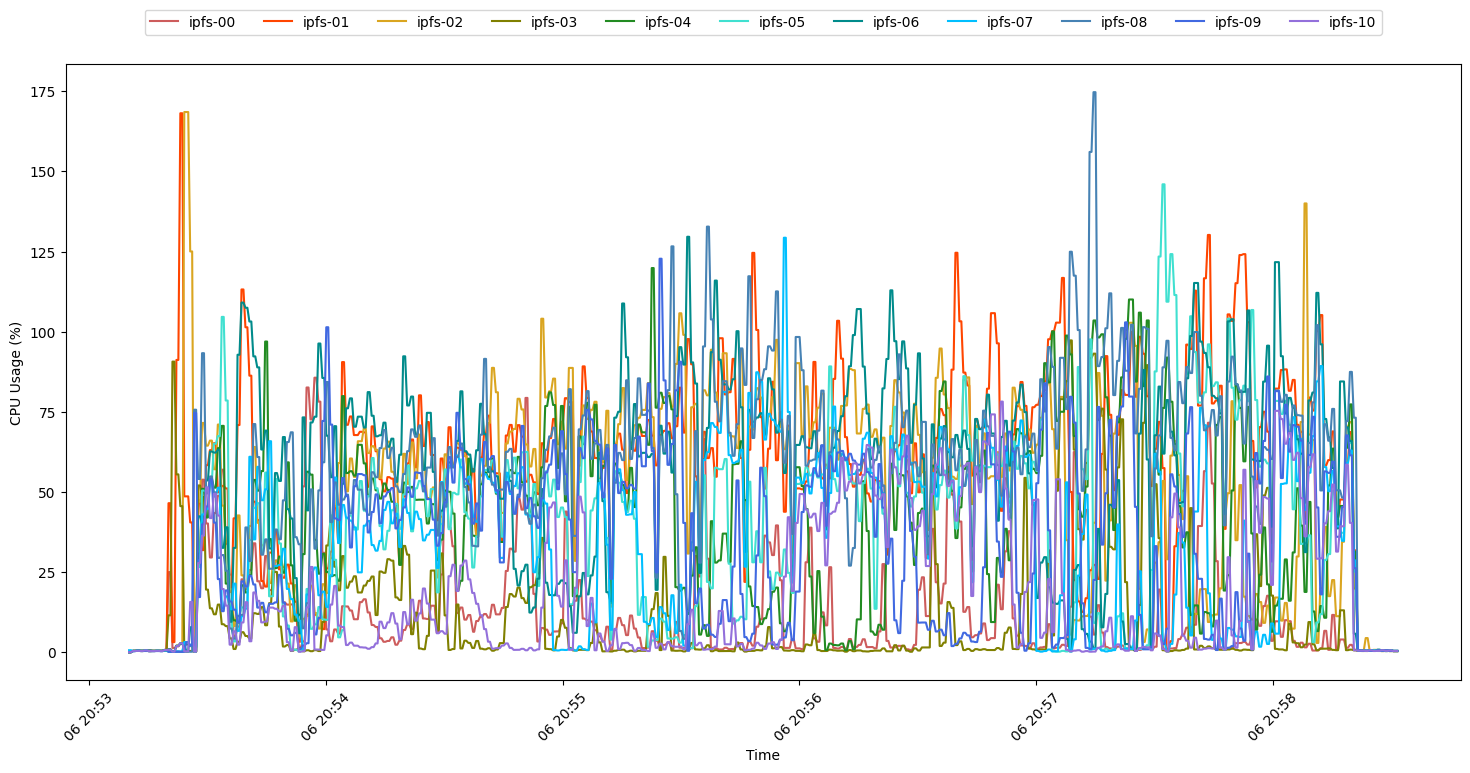
\includegraphics[width=\linewidth]{figures/graph-random/cpu_usage.png}
\caption{Random graph topology -- CPU usage}
\label{fig:graph-random-blk_read}
\end{figure}
\end{minipage}
\begin{minipage}{0.5\linewidth}
\begin{figure}[H]
\captionsetup{justification=centering,width=0.8\linewidth}
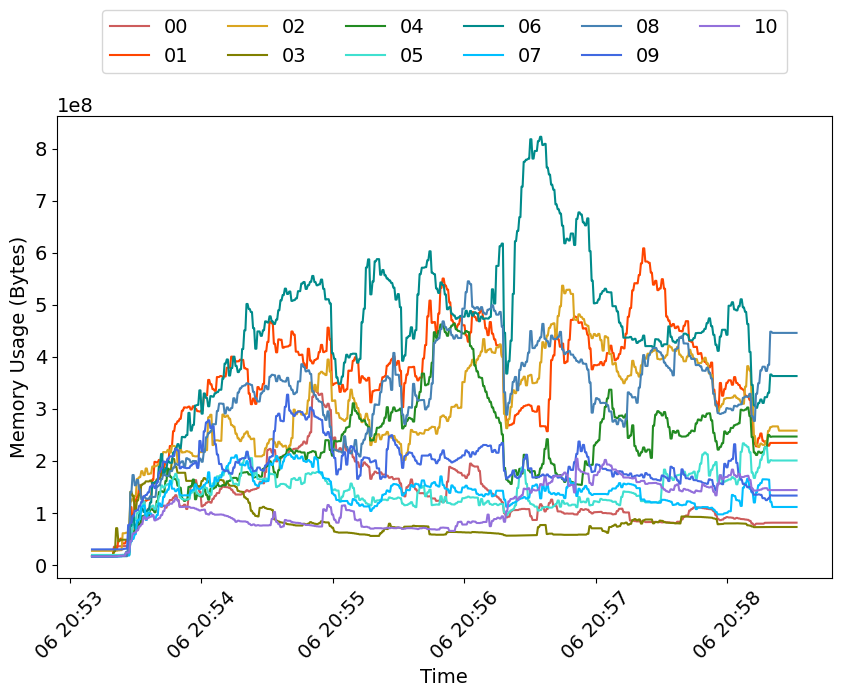
\includegraphics[width=\linewidth]{figures/graph-random/mem_usage.png}
\caption{Random graph topology -- memory usage}
\label{fig:graph-random-blk_write}
\end{figure}
\end{minipage}

\begin{minipage}{0.5\linewidth}
\begin{figure}[H]
\captionsetup{justification=centering,width=0.8\linewidth}
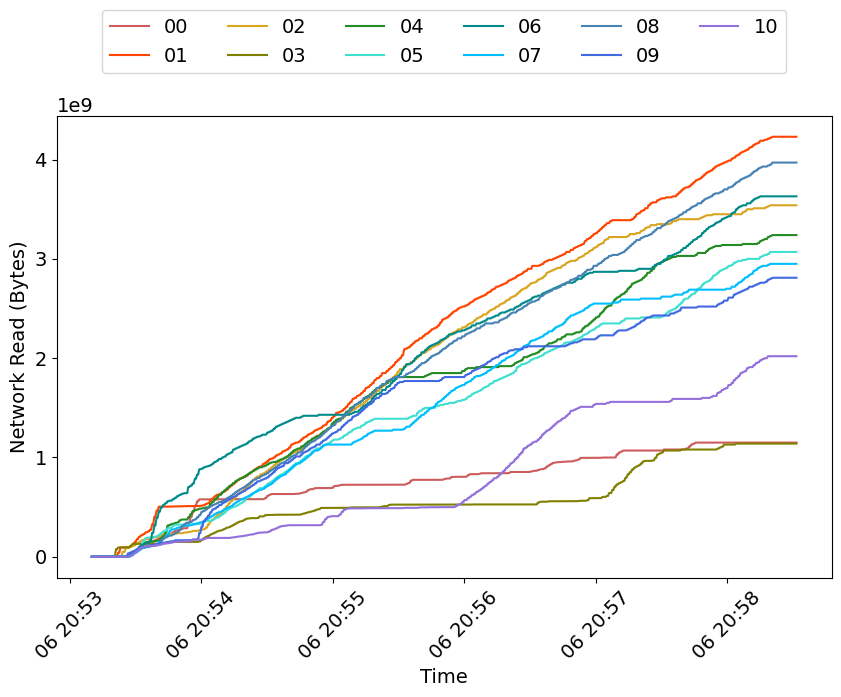
\includegraphics[width=\linewidth]{figures/graph-random/net_read.png}
\caption{Random graph topology -- amount of bytes received over network}
\label{fig:graph-random-cpu_usage}
\end{figure}
\end{minipage}
\begin{minipage}{0.5\linewidth}
\begin{figure}[H]
\captionsetup{justification=centering,width=0.8\linewidth}
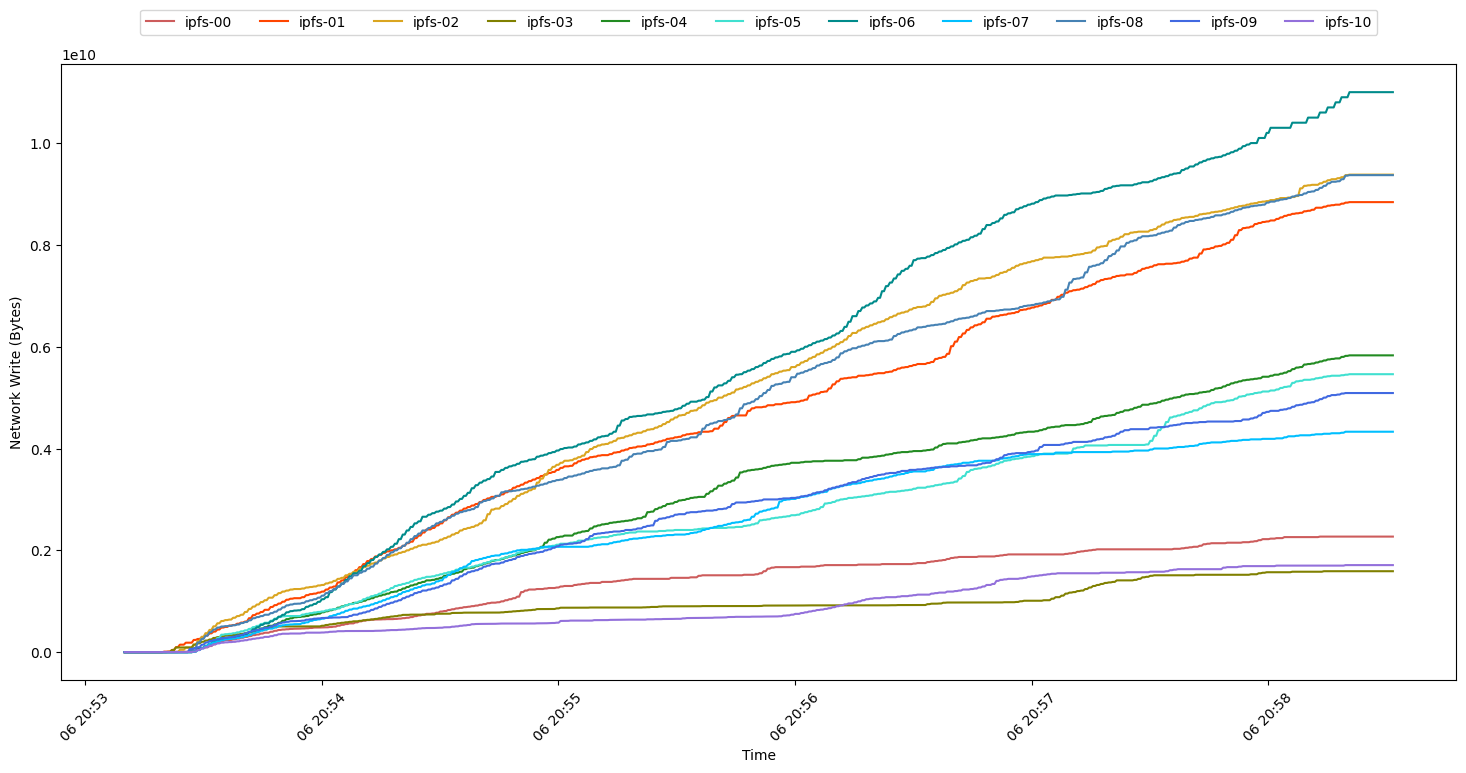
\includegraphics[width=\linewidth]{figures/graph-random/net_write.png}
\caption{Random graph topology -- amount of bytes sent over network}
\label{fig:graph-random-mem_usage}
\end{figure}
\end{minipage}

\begin{table}[H]
\begin{center}
\caption{Random graph -- metrics averages}
\label{tab:graph-random-avg}
\begin{tabular}{|c|c|c|c|c|c|c|}
\hline
   & CPU usage & Memory usage & Disk read & Disk write & Network read & Network write\\
\hline
00 & 12.90\% & 123.35 MiB & 3.41 MiB/s & 4.00 MiB/s & 4.19 MiB/s & 8.26 MiB/s\\
01 & 59.16\% & 335.59 MiB & 11.40 MiB/s & 14.23 MiB/s & 15.17 MiB/s & 31.69 MiB/s\\
02 & 51.43\% & 285.18 MiB & 9.49 MiB/s & 11.10 MiB/s & 12.84 MiB/s & 34.01 MiB/s\\
03 & 11.27\% & 81.31 MiB & 392.36 KiB/s & 4.23 MiB/s & 4.09 MiB/s & 5.70 MiB/s\\
04 & 41.28\% & 215.42 MiB & 8.12 MiB/s & 11.50 MiB/s & 11.79 MiB/s & 21.22 MiB/s\\
05 & 39.73\% & 132.86 MiB & 5.42 MiB/s & 10.29 MiB/s & 11.09 MiB/s & 19.72 MiB/s\\
06 & 55.55\% & 413.58 MiB & 14.47 MiB/s & 12.43 MiB/s & 12.97 MiB/s & 39.29 MiB/s\\
07 & 34.87\% & 128.90 MiB & 2.50 MiB/s & 10.66 MiB/s & 10.74 MiB/s & 15.76 MiB/s\\
08 & 58.58\% & 305.83 MiB & 10.73 MiB/s & 13.65 MiB/s & 14.34 MiB/s & 33.85 MiB/s\\
09 & 35.34\% & 176.26 MiB & 6.03 MiB/s & 10.12 MiB/s & 10.19 MiB/s & 18.46 MiB/s\\
10 & 19.33\% & 105.95 MiB & 1.51 MiB/s & 7.44 MiB/s & 7.30 MiB/s & 6.18 MiB/s\\
\hline
\end{tabular}
\end{center}
\end{table}

\begin{table}[H]
\begin{center}
\caption{Random graph -- metrics totals}
\label{tab:graph-random-total}
\begin{tabular}{|c|c|c|c|c|c|c|}
\hline
   & Disk read & Disk write & Network read & Network write\\
\hline
00 & 893.59 MiB & 1.02 GiB & 1.07 GiB & 2.11 GiB\\
01 & 2.96 GiB & 3.70 GiB & 3.94 GiB & 8.23 GiB\\
02 & 2.45 GiB & 2.85 GiB & 3.30 GiB & 8.74 GiB\\
03 & 102.04 MiB & 1.10 GiB & 1.06 GiB & 1.48 GiB\\
04 & 2.08 GiB & 2.94 GiB & 3.02 GiB & 5.43 GiB\\
05 & 1.40 GiB & 2.65 GiB & 2.86 GiB & 5.09 GiB\\
06 & 3.77 GiB & 3.24 GiB & 3.38 GiB & 10.24 GiB\\
07 & 655.17 MiB & 2.73 GiB & 2.75 GiB & 4.03 GiB\\
08 & 2.77 GiB & 3.52 GiB & 3.70 GiB & 8.73 GiB\\
09 & 1.56 GiB & 2.60 GiB & 2.62 GiB & 4.74 GiB\\
10 & 399.59 MiB & 1.92 GiB & 1.88 GiB & 1.59 GiB\\
\hline
\end{tabular}
\end{center}
\end{table}



\newpage
\subsection{Case 5: Complete Graph Topology}

\begin{wrapfigure}{r}{0.5\textwidth}
\centering
\captionsetup{justification=centering,width=0.8\linewidth}
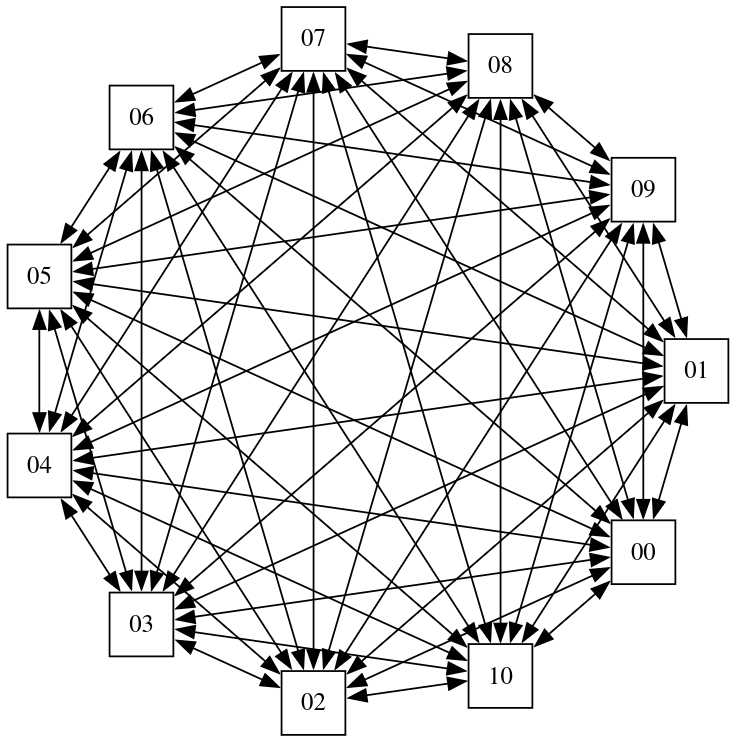
\includegraphics[width=0.7\linewidth]{figures/topologies/graph-complete.png}
\caption{Complete graph -- topology}
\label{fig:graph-complete-topology}
\end{wrapfigure}

Disk and network I/O is spread more or less evenly across nodes and are very
smooth, almost straight lines. CPU usage is the best among all topologies.
There are no nodes that are loaded more than others and they all and keep the
CPU usage very consistent start to finish at around 45\%. This is all thanks to
the fact that all nodes have all other nodes as neighbours, so they can
directly access the files on other instances without having to wait.

Figure \ref{fig:graph-complete-topology} displays how nodes are connected to
each other. Exact numbers for every metric are displayed in tables
\ref{tab:graph-complete-avg} and \ref{tab:graph-complete-total}. Table
\ref{tab:graph-complete-avg} contains metrics averages for every node.
Similarly, table \ref{tab:graph-complete-total} contains metrics totals for
every node.

\textcolor{white}{.}\\\\\\

\begin{minipage}{0.5\linewidth}
\begin{figure}[H]
\captionsetup{justification=centering,width=0.8\linewidth}
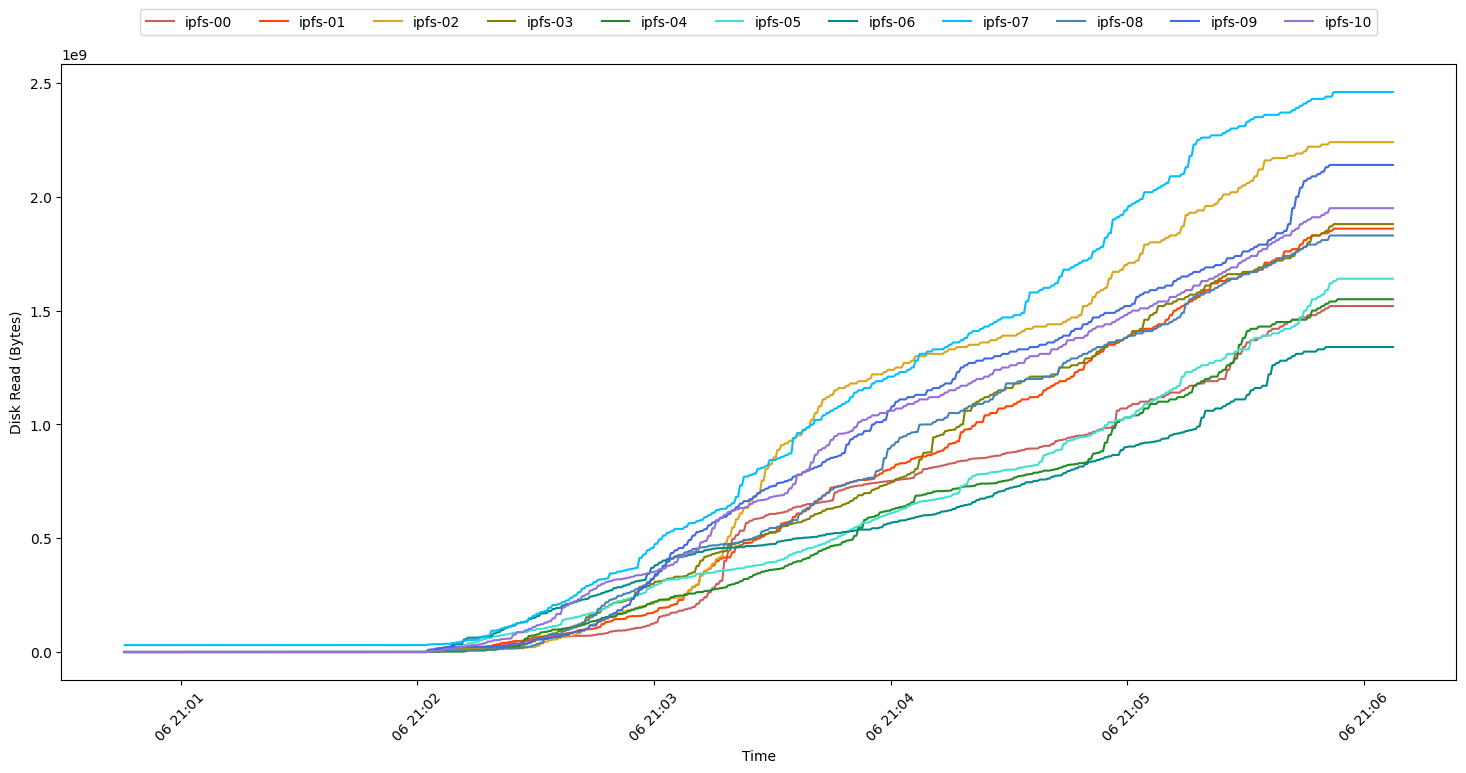
\includegraphics[width=\linewidth]{figures/graph-complete/blk_read.png}
\caption{Complete graph topology -- amount of bytes read from disk}
\label{fig:graph-complete-net_read}
\end{figure}
\end{minipage}
\begin{minipage}{0.5\linewidth}
\begin{figure}[H]
\captionsetup{justification=centering,width=0.8\linewidth}
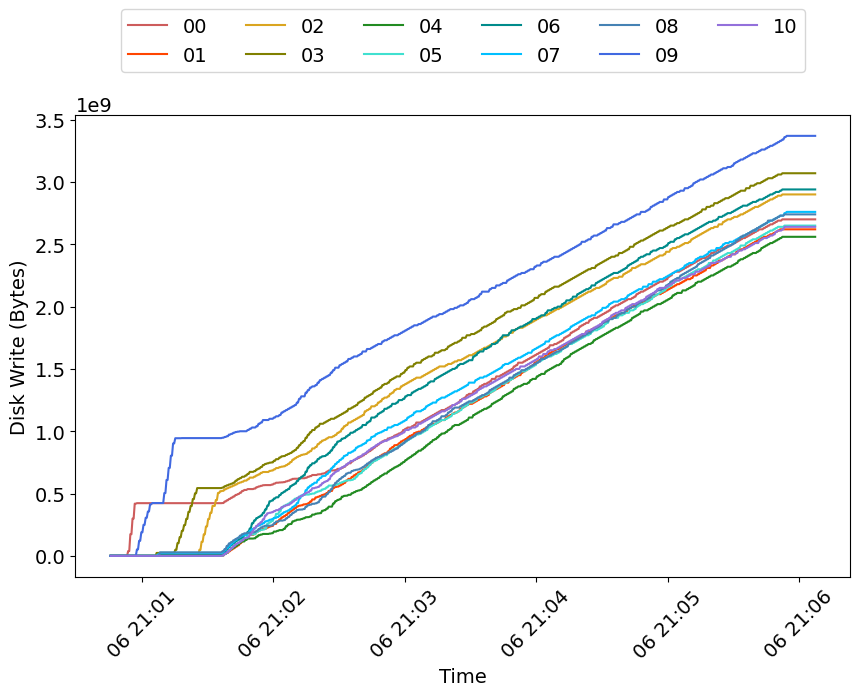
\includegraphics[width=\linewidth]{figures/graph-complete/blk_write.png}
\caption{Complete graph topology -- amount of bytes written to disk}
\label{fig:graph-complete-net_write}
\end{figure}
\end{minipage}

\begin{minipage}{0.5\linewidth}
\begin{figure}[H]
\captionsetup{justification=centering,width=0.8\linewidth}
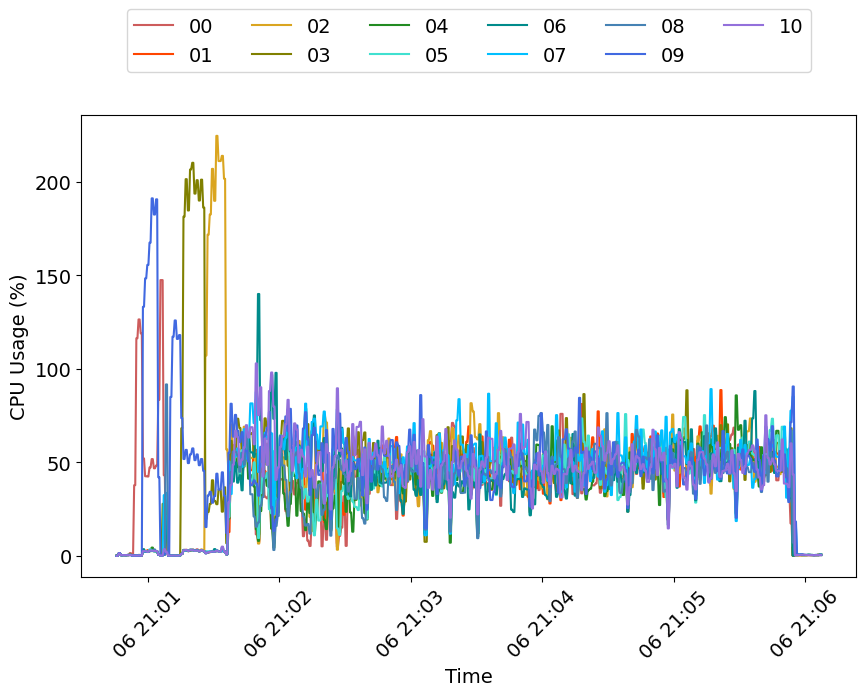
\includegraphics[width=\linewidth]{figures/graph-complete/cpu_usage.png}
\caption{Complete graph topology -- CPU usage}
\label{fig:graph-complete-blk_read}
\end{figure}
\end{minipage}
\begin{minipage}{0.5\linewidth}
\begin{figure}[H]
\captionsetup{justification=centering,width=0.8\linewidth}
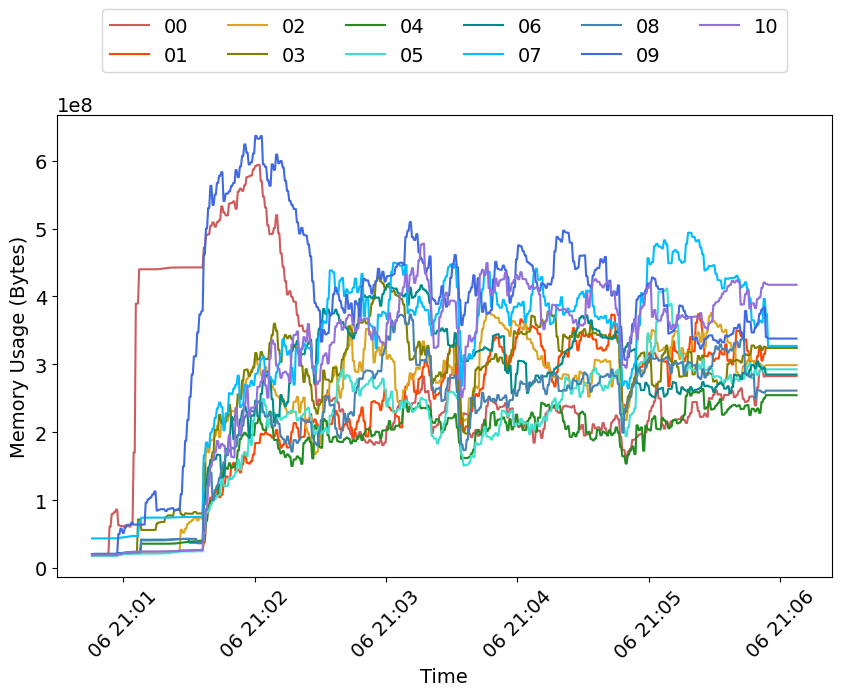
\includegraphics[width=\linewidth]{figures/graph-complete/mem_usage.png}
\caption{Complete graph topology -- memory usage}
\label{fig:graph-complete-blk_write}
\end{figure}
\end{minipage}

\begin{minipage}{0.5\linewidth}
\begin{figure}[H]
\captionsetup{justification=centering,width=0.8\linewidth}
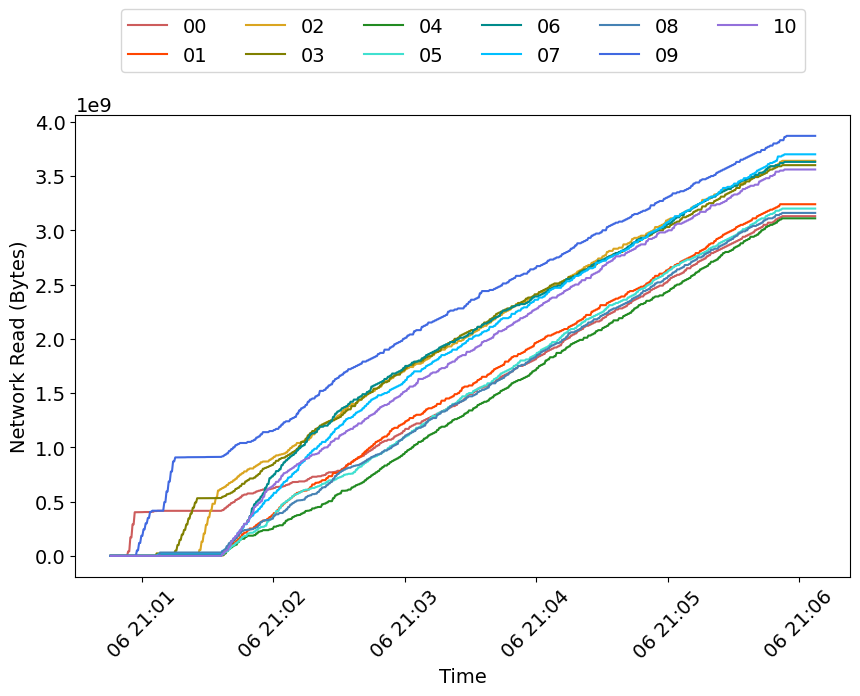
\includegraphics[width=\linewidth]{figures/graph-complete/net_read.png}
\caption{Complete graph topology -- amount of bytes received over network}
\label{fig:graph-complete-cpu_usage}
\end{figure}
\end{minipage}
\begin{minipage}{0.5\linewidth}
\begin{figure}[H]
\captionsetup{justification=centering,width=0.8\linewidth}
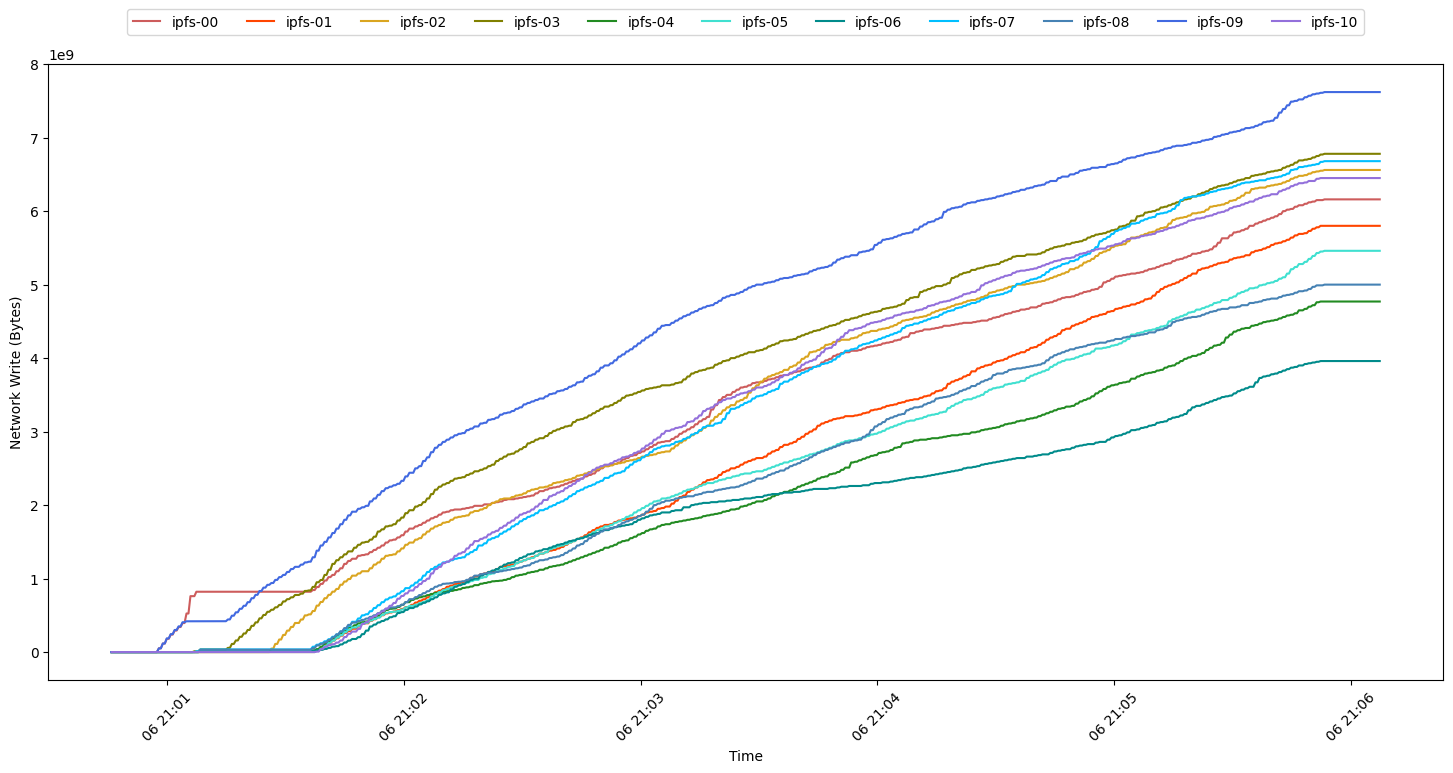
\includegraphics[width=\linewidth]{figures/graph-complete/net_write.png}
\caption{Complete graph topology -- amount of bytes sent over network}
\label{fig:graph-complete-mem_usage}
\end{figure}
\end{minipage}

\begin{table}[H]
\begin{center}
\caption{Complete graph -- metrics averages}
\label{tab:graph-complete-avg}
\begin{tabular}{|c|c|c|c|c|c|c|}
\hline
   & CPU usage & Memory usage & Disk read & Disk write & Network read & Network write\\
\hline
00 & 38.08\% & 266.04 MiB & 5.35 MiB/s & 9.50 MiB/s & 11.01 MiB/s & 21.68 MiB/s\\
01 & 38.12\% & 218.98 MiB & 6.59 MiB/s & 9.29 MiB/s & 11.49 MiB/s & 20.56 MiB/s\\
02 & 44.95\% & 238.56 MiB & 7.94 MiB/s & 10.28 MiB/s & 12.90 MiB/s & 23.26 MiB/s\\
03 & 47.01\% & 256.44 MiB & 6.71 MiB/s & 10.96 MiB/s & 12.86 MiB/s & 24.22 MiB/s\\
04 & 35.13\% & 170.07 MiB & 5.45 MiB/s & 9.01 MiB/s & 10.94 MiB/s & 16.79 MiB/s\\
05 & 37.39\% & 199.77 MiB & 5.77 MiB/s & 9.32 MiB/s & 11.26 MiB/s & 19.21 MiB/s\\
06 & 37.43\% & 249.37 MiB & 4.71 MiB/s & 10.35 MiB/s & 12.77 MiB/s & 13.94 MiB/s\\
07 & 43.06\% & 306.64 MiB & 8.58 MiB/s & 9.75 MiB/s & 13.07 MiB/s & 23.59 MiB/s\\
08 & 35.97\% & 213.71 MiB & 6.51 MiB/s & 9.75 MiB/s & 11.24 MiB/s & 17.79 MiB/s\\
09 & 48.82\% & 360.60 MiB & 7.53 MiB/s & 11.86 MiB/s & 13.62 MiB/s & 26.82 MiB/s\\
10 & 41.36\% & 290.04 MiB & 6.89 MiB/s & 9.32 MiB/s & 12.57 MiB/s & 22.78 MiB/s\\
\hline
\end{tabular}
\end{center}
\end{table}

\begin{table}[H]
\begin{center}
\caption{Complete graph -- metrics totals}
\label{tab:graph-complete-total}
\begin{tabular}{|c|c|c|c|c|c|c|}
\hline
   & Disk read & Disk write & Network read & Network write\\
\hline
00 & 1.42 GiB & 2.51 GiB & 2.92 GiB & 5.74 GiB\\
01 & 1.73 GiB & 2.44 GiB & 3.02 GiB & 5.40 GiB\\
02 & 2.09 GiB & 2.70 GiB & 3.39 GiB & 6.11 GiB\\
03 & 1.75 GiB & 2.86 GiB & 3.35 GiB & 6.31 GiB\\
04 & 1.44 GiB & 2.38 GiB & 2.90 GiB & 4.44 GiB\\
05 & 1.53 GiB & 2.47 GiB & 2.98 GiB & 5.09 GiB\\
06 & 1.25 GiB & 2.74 GiB & 3.38 GiB & 3.69 GiB\\
07 & 2.29 GiB & 2.57 GiB & 3.45 GiB & 6.22 GiB\\
08 & 1.70 GiB & 2.55 GiB & 2.94 GiB & 4.66 GiB\\
09 & 1.99 GiB & 3.14 GiB & 3.60 GiB & 7.10 GiB\\
10 & 1.82 GiB & 2.46 GiB & 3.32 GiB & 6.01 GiB\\
\hline
\end{tabular}
\end{center}
\end{table}



\subsection{Conclusion}

In this lab we had a detailed look at how Kubo's behaviour and performance
changes depending on the topology. Out of all topologies, the complete graph
performed the best. The behaviour was consistent across nodes with very smooth
disk and network I/O and more or less same load on every node. The complete
opposite of that was the ring topology, which performed the worst. The disk and
network usage was very uneven between nodes and CPU load was very spiky. We
think the main cause is that the ring topology makes it difficult to find a
file if it's not already on the node and also because files do not propagate
fast enough through the network. As a result many, clients just timeout while
running a query.

A general pattern became apparent, namely that the more neighbours a node has,
the higher the chance that the node will be able to find the file in the
network. This was made very obvious in random graph topology where nodes with
most neighbours are able to serve a bigger chunk of queries compared to nodes
with just one or two neighbours.

In our experiments, the original implementation connects all nodes in a
complete graph, but that is probably because there are not enough nodes to
simulate real life connection behaviour. In reality, having a complete graph
wouldn't scale well, so at some point the topology would start to look closer
to a random graph as in Case 4 and exhibit similar performance characteristics.


\end{document}
